\newcommand\abs[1]{\ensuremath{\left|#1\right|}}

\def\be{\begin{equation}}
\def\ee{\end{equation}}

\def\bea{\begin{eqnarray}}
\def\eea{\end{eqnarray}}

\def\Msun{M_\odot}

\def\cross{\times}


%\eads{\mailto{} \mailto{}}



\acrodef{aLIGO}[aLIGO]{Advanced Laser Interferometer Gravitational-wave Observatory}
\acrodef{AdV}[AdV]{Advanced Virgo}
\acrodef{LIGO}[LIGO]{Laser Interferometer Gravitational-wave Observatory}
\acrodef{CBC}[CBC]{compact binary coalescence}
\acrodef{S6}[S6]{LIGO's sixth science run}
\acrodef{VSR23}[VSR2 and VSR3]{Virgo's second and third science runs}
\acrodef{EM}[EM]{electromagnetic}
\acrodef{NS}[NS]{neutron star}
\acrodef{BH}[BH]{black hole}
\acrodef{BNS}[BNS]{binary neutron star}
\acrodef{NSWD}[NSWD]{neutron star-white dwarf}
\acrodef{NSBH}[NSBH]{neutron star and a black hole}
\acrodef{GRB}[GRB]{gamma-ray burst}
\acrodef{S5}[S5]{LIGO's fifth science run}
\acrodef{S4}[S4]{LIGO's fourth science run}
\acrodef{VSR1}[VSR1]{Virgo's first science run}

\acrodef{PSD}[PSD]{power spectral density}
\acrodef{VSR3}[VSR3]{Virgo's third science run}
\acrodef{BBH}[BBH]{binary black holes}
\acrodef{SNR}[SNR]{signal-to-noise ratio}
\acrodef{SPA}[SPA]{stationary-phase approximation}
\acrodef{LHO}[LHO]{LIGO Hanford Observatory}
\acrodef{LLO}[LLO]{LIGO Livingston Observatory}
\acrodef{LSC}[LSC]{LIGO Scientific Collaboration}
\acrodef{PN}[PN]{post-Newtonian}
\acrodef{DQ}[DQ]{data quality}
\acrodef{IFO}[IFO]{interferometer}
\acrodef{DTF}[DTF]{detection template families}
\acrodef{FAR}[FAR]{false alarm rate}
\acrodef{FAP}[FAP]{false alarm probability}
\acrodef{PTF}[PTF]{physical template family}
\acrodef{ADE}[ADE]{advanced detector era}
\acrodef{FFT}[FFT]{Fast Fourier Transformation}
\acrodef{GPU}[GPU]{graphical processing unit}
\acrodef{ISCO}[ISCO]{inner-most stable circular orbit}
\acrodef{MECO}[MECO]{minimum energy circular orbit}

\section{Introduction}
\label{sec:introduction}

In this chapter we investigate if the currently available post-Newtonian models
are sufficient for use in searches for gravitational-waves from the
coalescence of a neutron star and a black hole. Given the uncertainties in the masses and spins of
\ac{NSBH} binaries, we consider a fairly broad mass and spin
distribution when investigating the accuracy of \ac{NSBH} waveforms.
In this chapter, we consider \ac{NSBH} binaries with the \ac{NS} mass between 1
and $3\, M_\odot$, the \ac{BH} mass between $3$ and $15\, M_\odot$, the
\ac{NS} spin between 0 and $0.05$ and the
\ac{BH} spin between 0 and 1. Between these limits, the distributions of mass and spin are all
assumed to be uniform. 


As described in Ch.\ref{ch:sources}, there are several different ways in which to solve the energy balance equation
to obtain the gravitational-wave phase measurable by aLIGO; these different methods are known as
\ac{PN} \emph{approximants.} While the convergence of the full \ac{PN} series 
is not guaranteed, for \ac{BNS} systems in Advanced LIGO, the
available \ac{PN} approximants produce waveforms that are indistinguishable for
a given binary and are reliable for use in detection searches and parameter
measurement~\cite{Simone:1996db,Buonanno:2009zt,Brown:2012qf}. However, for \ac{NSBH}
binaries the total mass, and hence the \ac{PN} expansion parameter $v$, is
larger. The mass ratio and spin corrections are also more significant. 
We investigate the accuracy of 
waveforms generated by different \ac{PN} approximants for observing \ac{NSBH}
binaries with aLIGO.
To do this, one could compare subsequent terms in the \ac{PN} expansion and
determine the effect of neglecting them. However, in the case of systems whose
component objects are spinning, only terms up to 2.5\ac{PN} order are
completely known~\cite{Kidder:1992fr,Kidder:1995zr,Arun:2008kb}. 
This represents the leading order (1.5\ac{PN}) and
next-to-leading order (2.5\ac{PN}) spin-orbit, along with the leading order
(2.0\ac{PN}) spin-spin contributions to the phasing~\cite{Kidder:1992fr,Kidder:1995zr,Arun:2008kb}.  
We choose to compare approximants that are constructed with terms up to the same
\ac{PN} order, but that use inversely related differential equations to solve
for the orbital dynamics, in addition to comparing to approximants that include
higher order spin-related corrections at partially derived orders~\cite{Bohe:2013cla, Blanchet:2011zv}.
These methods both have the effect of testing
how well the \ac{PN} series has converged. We also present a comparison between
waveforms from these \ac{PN} approximants where we fix the mass and spin
parameters of the objects in order to understand when in the inspiral the waveforms diverge.

We consider two families of \ac{PN} approximants for binaries where the spin
of the black hole is aligned with the orbital angular momentum:
TaylorT2~\cite{Blanchet:1996pi, Droz:1999qx, Blanchet:2006zz} and
TaylorT4~\cite{Buonanno:2002fy}.  In these models, we include all the
completely known orbital evolution terms (up to 3.5\ac{PN} order)~\cite{Wiseman:1993aj,Blanchet:1995fg,Blanchet:1995ez,Blanchet:1996pi,
Blanchet:2001ax, Blanchet:2004ek} and all the
completely known spin-related terms (up to 2.5\ac{PN}
order)~\cite{Faye:2006gx, Blanchet:2006gy, Kidder:1992fr, Mikoczi:2005dn,
Racine:2008kj}.  Restricting to systems where the spin angular momenta are
aligned (or anti-aligned) with the orbital angular momentum means that the
plane of the binary does not precess, simplifying our comparisons. However,
this study captures the dominant effect of spin on the
waveforms~\cite{Brown:2012gs}. In Ch.~\ref{ch:nsbh_prec}, we investigate the effect
of precession on detection searches~\cite{Harry:2013tca}.
We also consider the
effective-one-body model as described in Ref.~\cite{Taracchini:2012ig}. 
We restrict to comparing the inspiral portion of approximants. Even at the upper 
range of masses we consider, $(3+15)M_{\odot}$, it has been shown in the case of numerically modelled 
binary black hole waveforms that inspiral-only
template banks recover $> 95\%$ of the signal power~\cite{Brown:2012nn, Smith:2013mfa}.
We separately consider models that include
spin-related terms up to 3.5\ac{PN} order~\cite{Bohe:2013cla,
Blanchet:2011zv}. Spin-orbit tail (3.0\ac{PN}) and next-to-next-to-leading
order spin-orbit (3.5\ac{PN}) contributions to the phasing are known.
However, these orders are incomplete as there are also unknown spin
corrections at 3.0\ac{PN} and 3.5\ac{PN}, including spin-spin and
(spin-induced) octupole-monopole couplings. 

In Fig.~\ref{fig:t4horizon} we show  
the distance an optimally oriented system would be observed at \ac{SNR} 8 (the horizon distance),
for a $1.4\Msun-10\Msun$ \ac{NSBH} system, as a function of the spin of the
black hole, for both the \ac{aLIGO} zero-detuned, high-power sensitivity curve and a
plausible range of early \ac{aLIGO} sensitivities~\cite{Aasi:2013wya}. 
Systems where the spin of the black hole is large in magnitude and aligned with the orbital 
angular momentum can be seen from a greater distance than systems where the spin is 
small or anti-aligned. Achieving this sensitivity requires \ac{NSBH} waveforms that do not
incur a significant loss in \ac{SNR} when used as search templates ~\cite{Apostolatos:1996rf}.
Furthermore, extracting the physics from observed signals requires faithful templates for parameter measurement.

We find that no presently available waveform model is sufficiently accurate for use
in \ac{aLIGO} \ac{NSBH} searches or parameter measurement. Our key results, Figs.~\ref{fig:f2f4f}-\ref{fig:seobnrf},
show the match between the various waveform families considered here.
There is a significant disagreement between the \ac{PN} approximants we
have examined, even at at low ($\chi \sim 0.4$) spins and small ($m_{BH}/m_{NS} \sim 4$) mass ratios for TaylorF2 and TaylorT4.
The match decreases as these increase with matches as low as $\sim 0.1$ observed. This motivates
the need to compute higher order \ac{PN} spin corrections.  

Our present knowledge of \ac{NSBH} waveforms will limit the
ability of gravitational-wave observatories to accurately determine source
parameters from the detected signals and may hinder their detection.
Further analytical and numerical modeling of \ac{NSBH} systems will be needed
before \ac{aLIGO} comes online in 2015 and reaches full sensitivity in $\sim$
2019~\cite{Aasi:2013wya}.

The remainder of this chapter is organized as follows.  In
Sec.~\ref{sec:waveforms}, we describe the construction of the \ac{PN}
approximants used and Sec.~\ref{sec:faithfulness_definition} describes our
method of comparing them.  In Sec.~\ref{sec:faithfulness} we show the results
of comparing different \ac{PN} approximants, and show that there is a large
discrepancy between the waveforms for \ac{NSBH} binaries at relatively low
black hole spins. In Sec.~\ref{sec:R2F4} we construct a new frequency domain
approximant that is designed to agree with TaylorT4. This is followed by a
comparison of the time domain approximants to their frequency domain
counterparts in Sec.~\ref{sec:freq_vs_time_approx}, where we demonstrate that
they largely agree. Finally, in Sec.~\ref{sec:faithfulness_phase} and
Sec.~\ref{sec:faithfulness_match_accumulation} we investigate where in the
inspiral the disagreement between the waveform families becomes important. We
demonstrate that the divergence occurs at surprisingly low velocities for even
modest black hole spins. Finally in Sec.~\ref{sec:effectualness_and_flow} we
investigate whether maximizing over the mass and spin parameters of the
waveform can improve present models, and investigate the accuracy of the
waveforms for early aLIGO observations when the detectors will have reduced
low-frequency sensitivity when compared to the ultimate sensitivity. 

%%%%%%%%%
%\section{Observational Mass and Spin Distributions}
%\label{sec:dist}


\begin{figure}
\begin{center}
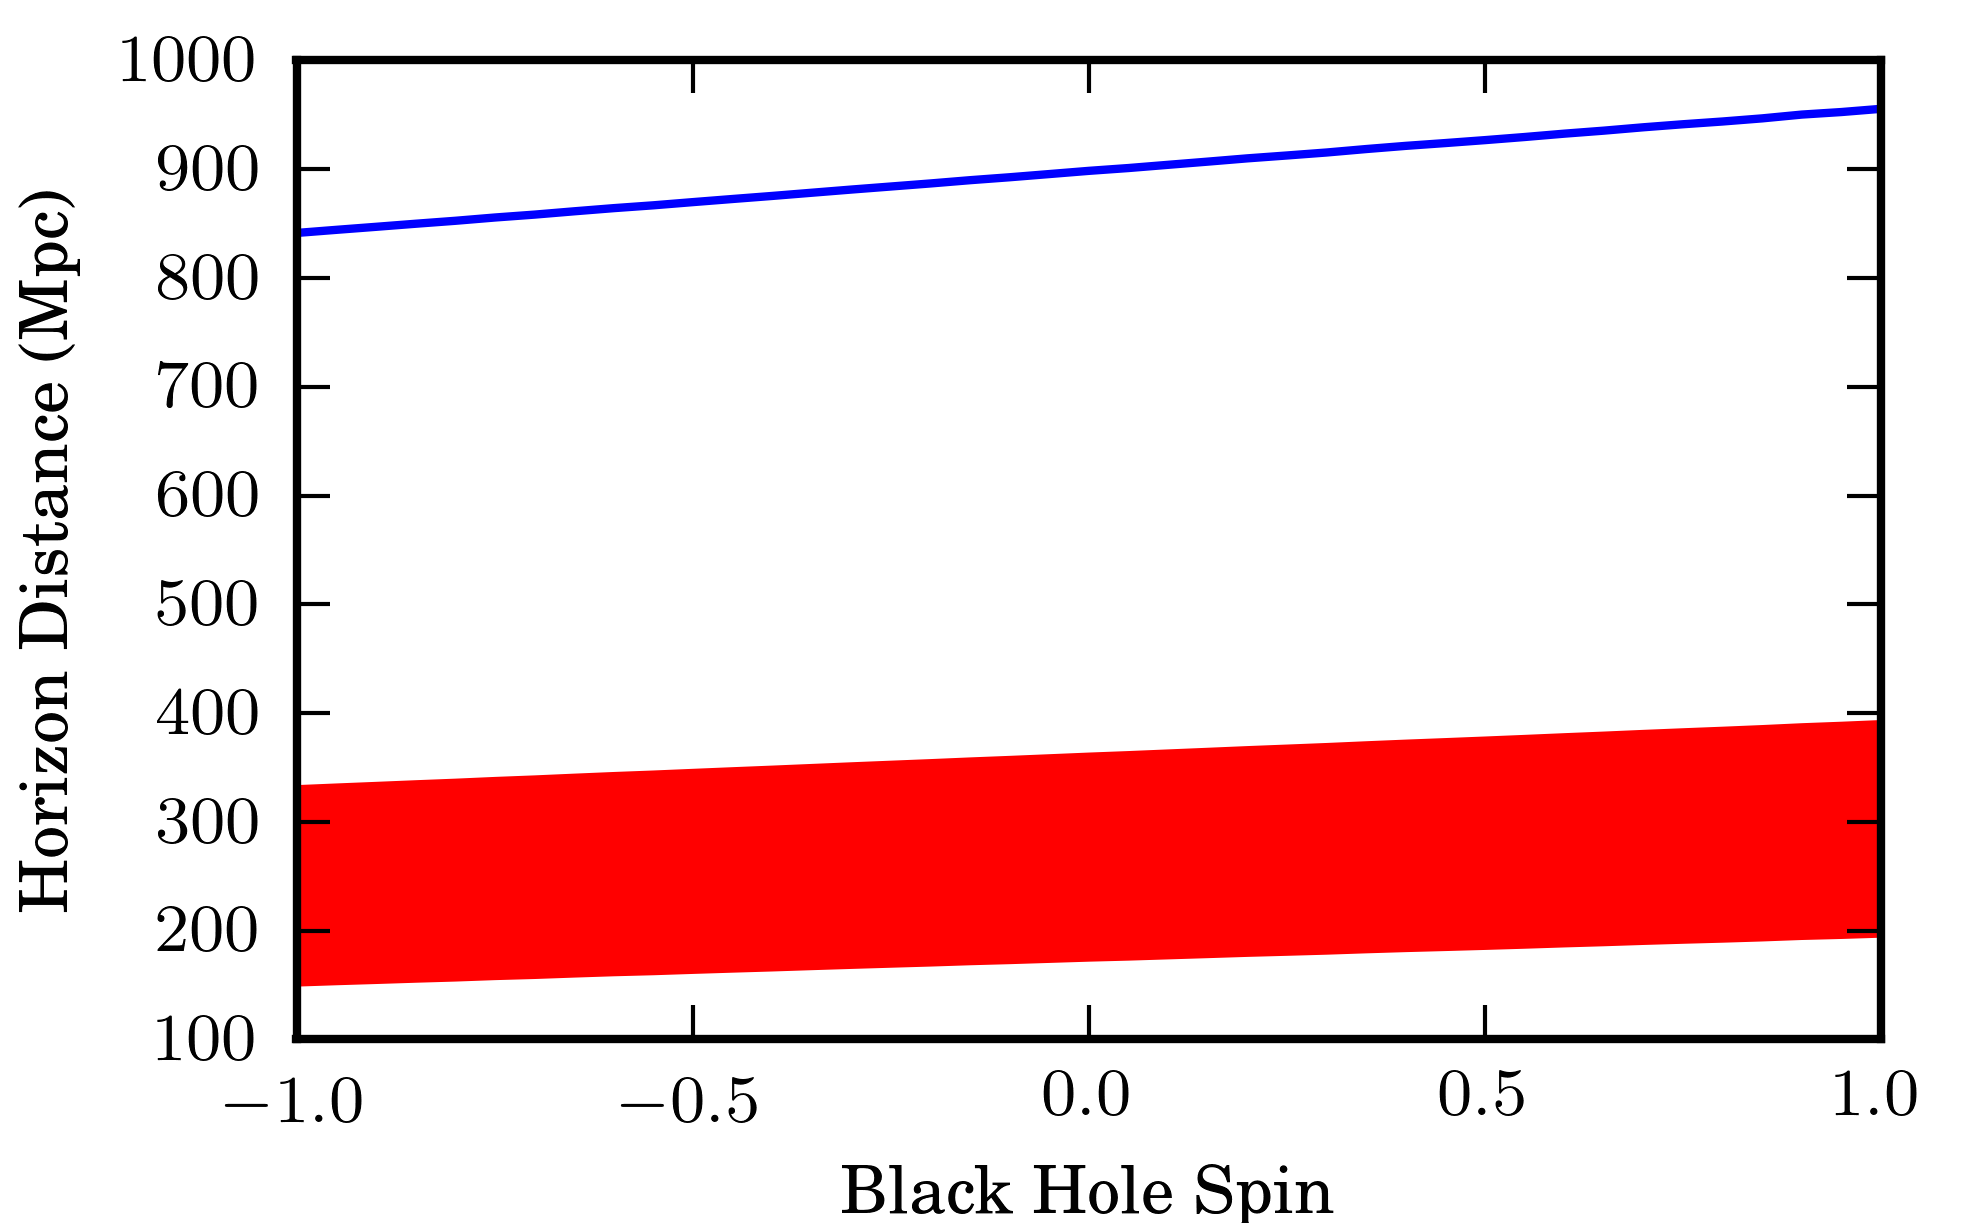
\includegraphics[width=1.0	\textwidth]{papers/nsbh_faithfulness/figure1.png}
\end{center}
\caption{\label{fig:t4horizon} 
The horizon distance as a function of the spin of the black hole 
for a $1.4\Msun-10\Msun$ \ac{NSBH} system, for both the \ac{aLIGO} zero-detuned,
high-power aLIGO sensitivity curve (blue) and plausible early \ac{aLIGO}
detector sensitivities (red), with a 15 Hz lower frequency cutoff. 
Results are obtained using the TaylorT4 approximant including only the 
complete spin terms up to 2.5\ac{PN}. Note that \ac{aLIGO} will be sensitive to
\ac{NSBH} systems out to $\sim 900$ Mpc, and there will be increased sensitivity
for systems with aligned black hole spins with large magnitudes. 
}
\end{figure}


%%%%%%%%
\section{Post-Newtonian approximant faithfulness comparison}
\label{sec:faithfulness}

\begin{figure}
\begin{center}
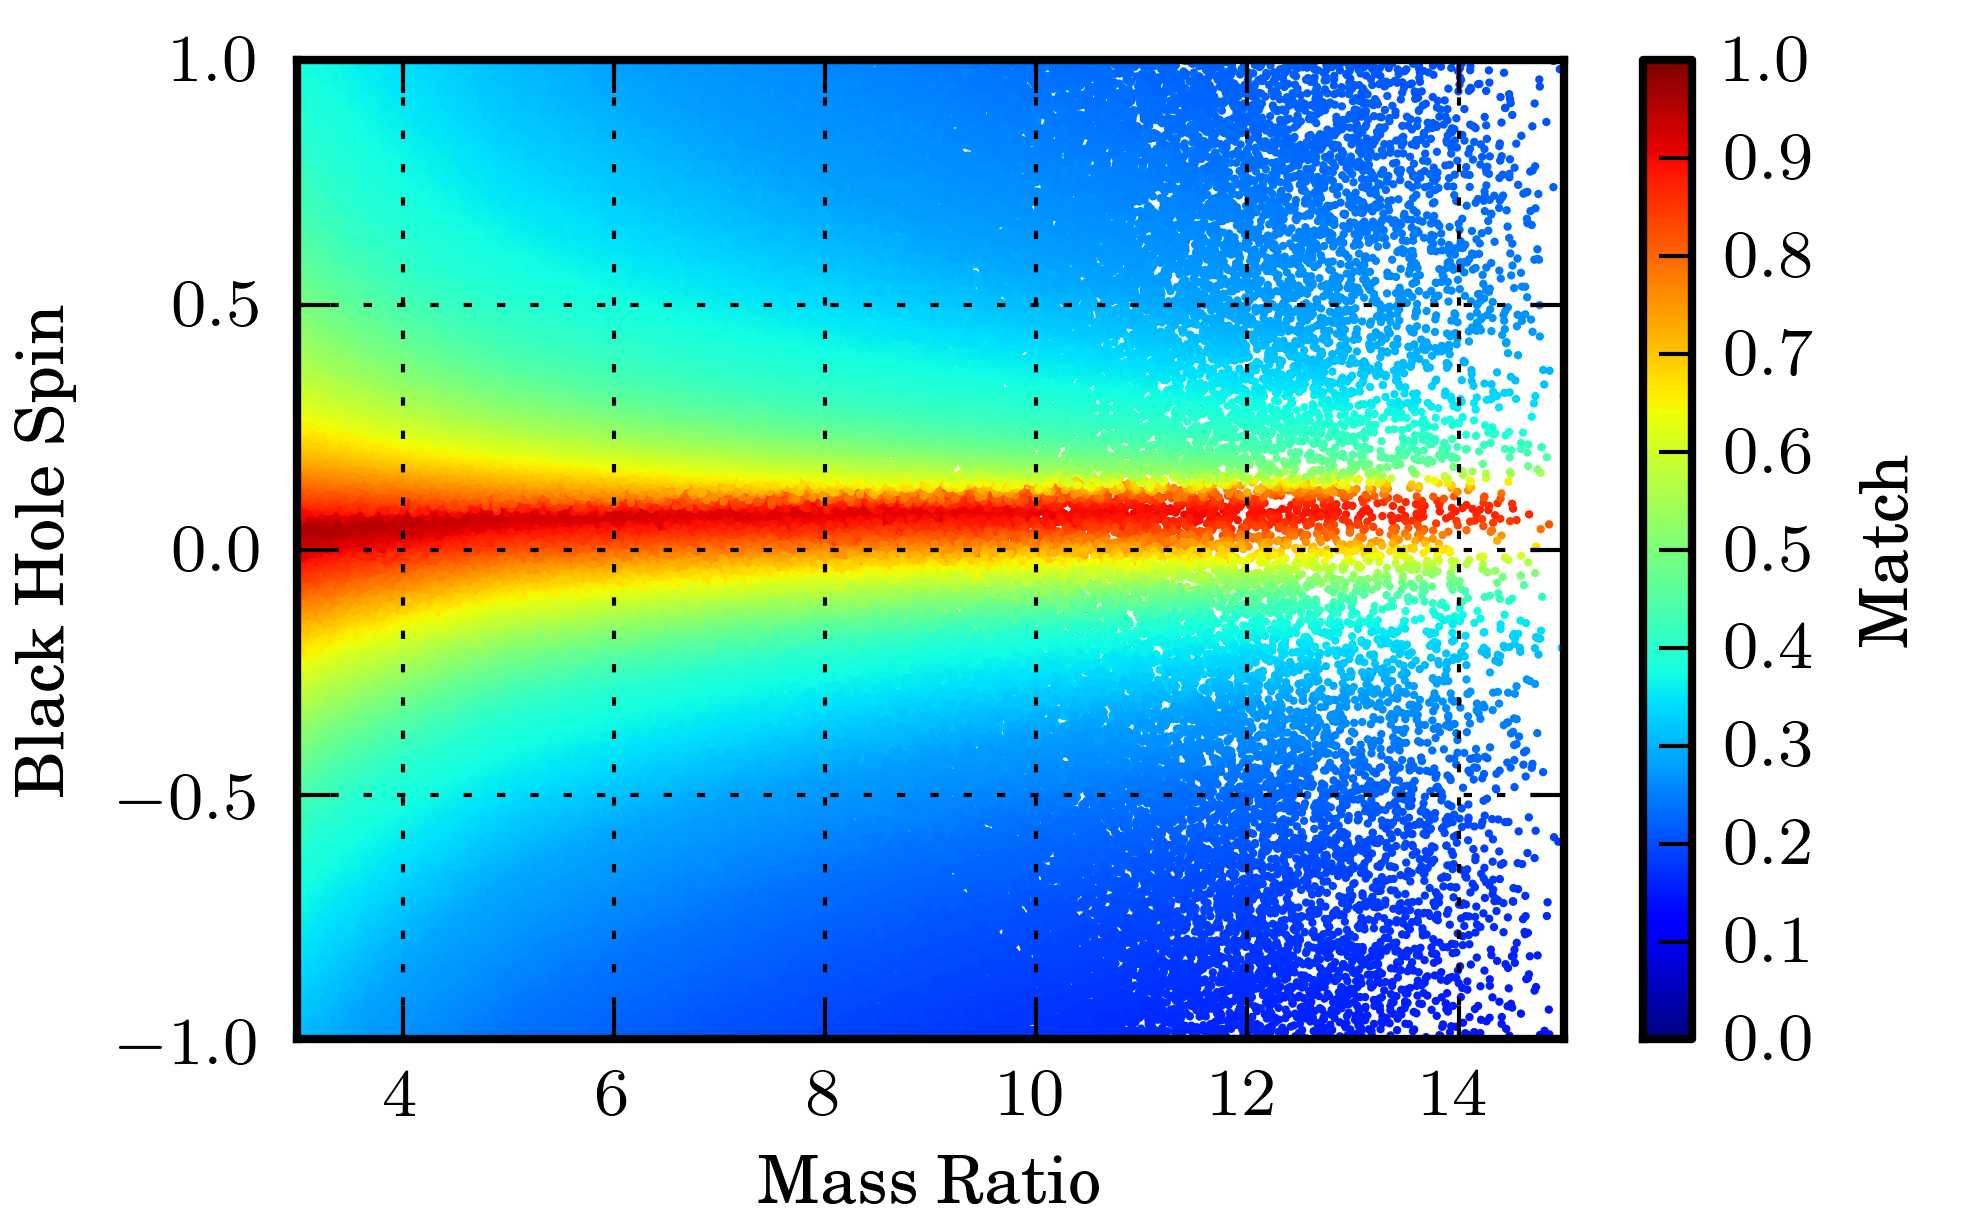
\includegraphics[width=1.0	\textwidth]{papers/nsbh_faithfulness/figure2.png}
\end{center}
\caption{\label{fig:f2f4f}The match between the TaylorF2 and
TaylorT4 approximants as a function of the spin of the black hole
and the mass ratio of the system. Only the completely known 
spin-related corrections up to 2.5\ac{PN} are included. Matches are calculated using the
the aLIGO zero-detuned, high-power sensitivity curve and a 15Hz lower frequency cutoff.
A significant reduction in match is seen for even moderate spins $\chi \sim 0.3$
and low mass ratios $m_{bh}/m_{ns} \sim 4$. The approximants also begin to disagree for non-spinning
systems as the mass ratio increases.
}


\end{figure}

\begin{figure}
\begin{center}
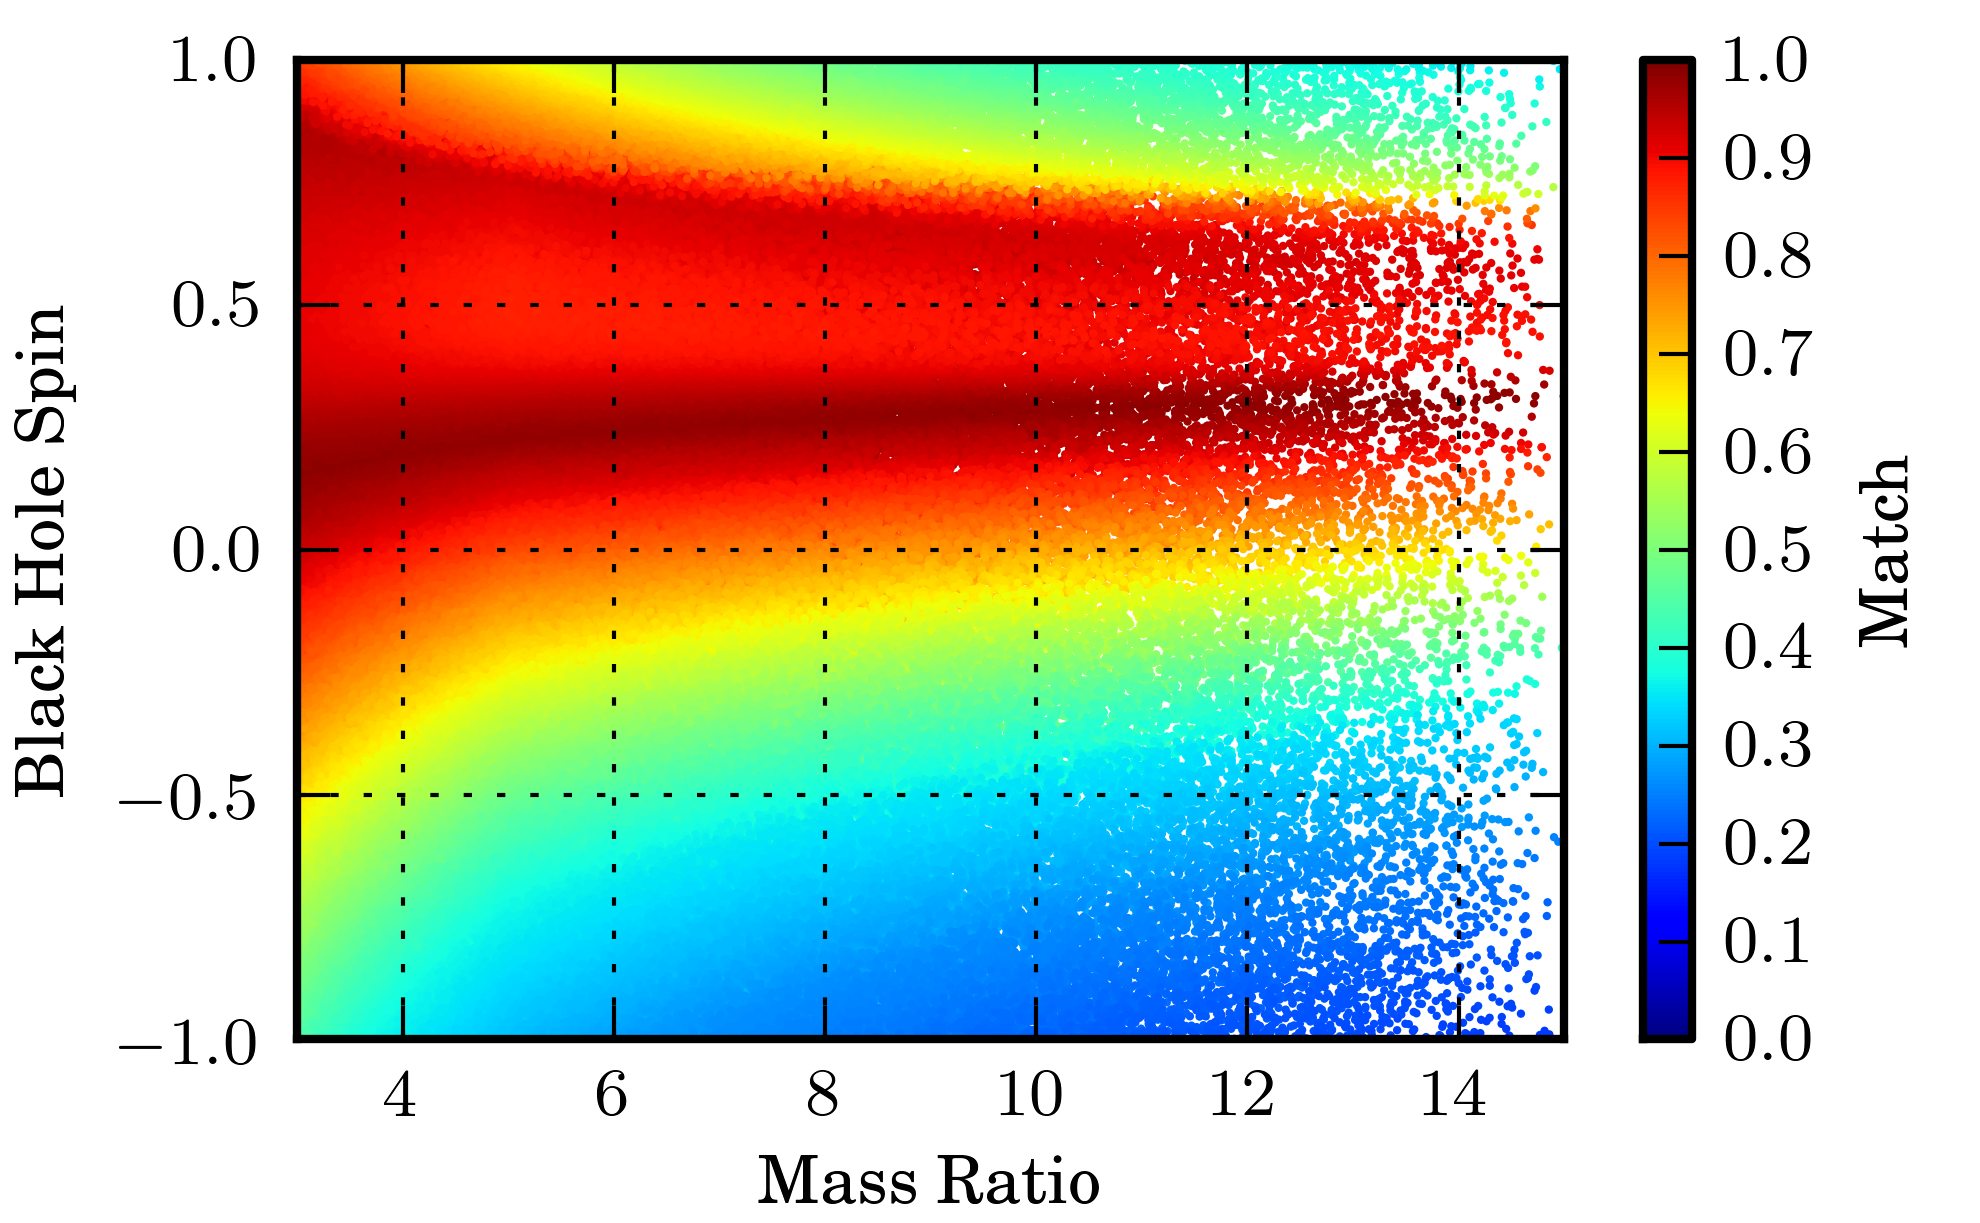
\includegraphics[width=1.0	\textwidth]{papers/nsbh_faithfulness/figure3.png}
\end{center}
\caption{\label{fig:f2t4fso}The match between the TaylorF2 and TaylorT4 approximants
as a function of black hole spin and mass ratio. Both models include
the next-to-next-to-leading spin-orbit (3.5\ac{PN}) and spin-orbit tail 
terms (3.0\ac{PN}). In comparison to Fig. \ref{fig:f2f4f}, the additional terms have 
improved the agreement for moderately spinning aligned spin systems, however, the
match is still $ \sim 0.8 $ for $\chi \sim 0.5 $ at all mass ratios.}

\end{figure}

Searches for gravitational waves from compact binary coalescences utilize
matched-filtering~\cite{Wainstein,Allen:2005fk}, in which the signal model is
correlated with the detector output to construct a signal-to-noise
ratio. If the signal model does not accurately capture the true gravitational
waveform, then the signal-to-noise ratio, and hence the distance to which the
detector can see signals at a given false alarm rate, will decrease. Matched-filtering 
therefore relies on the accuracy of the models. We quantify the 
agreement between waveform families by computing the match, or
\emph{faithfulness} of the waveforms.

The \emph{faithfulness} of representing a waveform from a given \ac{PN} family with
that of another is described by the match between the two waveforms when the
same physical parameters are used as input to the models. As both models
describe the same physical source, the match should be unity. Any deviation is
due to the variation between models and the match gives the fractional loss in
signal-to-noise ratio that will result.

In this section we compare the faithfulness between waveforms from different
\ac{PN} approximants where we choose the physical parameters to be consistent
with \ac{NSBH} sources.  We also consider how the waveforms from the \ac{PN}
approximants compare to the waveforms from the SEOBNRv1 effective-one-body
model~\cite{Taracchini:2012ig}. Lastly, we consider the effect of including 
the spin-related terms at only partially derived orders. 
We model the sensitivity of second generation  gravitational-wave detectors with the aLIGO
zero-detuned, high-power sensitivity curve~\cite{aLIGOSensCurves}. For this
study we use a lower frequency cutoff of 15Hz since it is not expected that
detectors will have significant sensitivity below this frequency. We consider
the effect of increasing this low-frequency cutoff to simulate early aLIGO
sensitivities in Sec.~\ref{sec:effectualness_and_flow}.

In Fig.~\ref{fig:f2f4f}, we examine the faithfulness of \ac{NSBH} waveforms by computing the match between the TaylorF2 and TaylorT4 \ac{PN} approximants.
The TaylorT4 approximant was used to simulate \ac{NSBH} binaries in LIGO's
previous gravitational-wave searches, and the TaylorF2 family is used as the
templates for detection~\cite{Abadie:2011nz}.
In order to focus
on the mismatches primarily due to phase differences between the models, the
frequency cutoff of the TaylorF2 waveform is made to agree with the ending
frequency of the TaylorT4 waveform. We see that the agreement between the two
models is primarily influenced by the magnitude of the black hole's spin, and
secondarily by the mass ratio. There is a noticeable drop in match at higher
mass ratios, even when
the spin of the black hole is zero. As expected, the best
agreement is seen when the black hole's spin is small and
the black hole and neutron star have comparable masses.
However, this plot shows that there is a \emph{substantial} disagreement between
these approximants for even moderately low black hole spins ($\chi \sim 0.3$),
which increases as the spin of the black hole increases. 
We note that the effect on the match due to the spin of the
neutron star is negligible in all areas.  In Fig.~\ref{fig:f2t4fso} we compare
the TaylorF2 and TaylorT4 models, with the inclusion of the spin-orbit
tail (3.0\ac{PN}) and next-to-next-to-leading spin-orbit (3.5\ac{PN})
corrections recently computed in Refs.~\cite{Bohe:2012mr, Blanchet:2012sm}.  In comparison to
Fig.~\ref{fig:f2f4f}, the agreement is improved for aligned spins
with moderate magnitudes. However, these approximants maintain a poor level of
overall agreement, with matches of only $\sim 0.8$ at $\chi \sim 0.5$ for all mass ratios, and even
lower matches for anti-aligned systems. 
Figs.~\ref{fig:5715f2f2} and~\ref{fig:5715t4t4} compare the TaylorT2 and TaylorT4 approximants with and without
these additional spin terms.
We see that TaylorT4 is especially sensitive to the additional corrections.
In both cases, however, we note that the additional terms have caused a significant change in the waveforms, 
as indicated by the low matches, demonstrating that the expansion has
not yet sufficiently converged to produce reliable waveforms for parameter estimation. 

\begin{figure}
\begin{center}
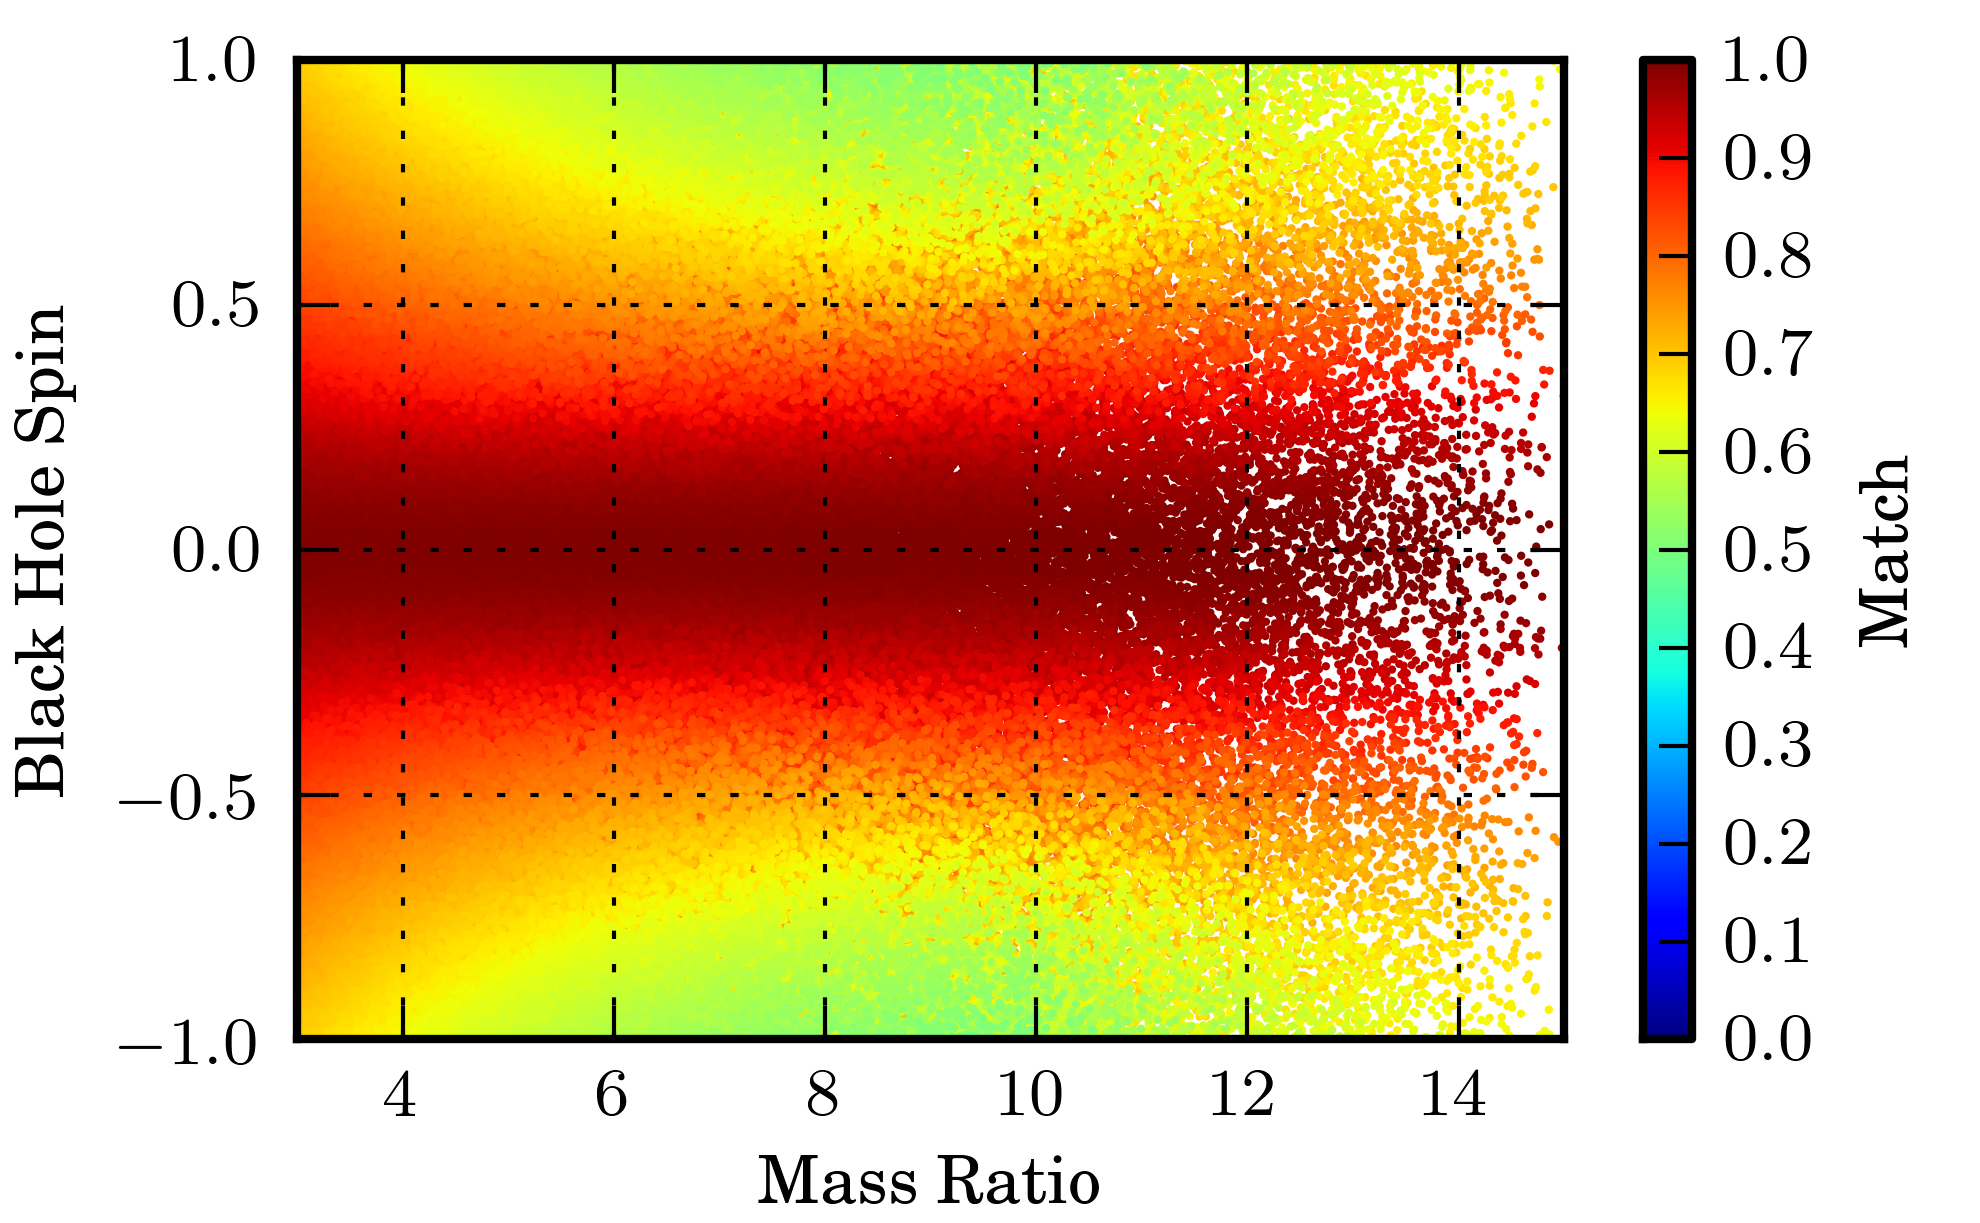
\includegraphics[width=1.0	\textwidth]{papers/nsbh_faithfulness/figure4.png}
\end{center}
\caption{\label{fig:5715f2f2}The match between TaylorF2 with 2.5\ac{PN} spin corrections
and TaylorF2 including the next-to-next-to-leading spin-orbit (3.5\ac{PN}) and spin-orbit tail 
terms (3.0\ac{PN}), as a function of the spin of the black hole
and the mass ratio of the system. Matches are calculated using the the aLIGO
zero-detuned, high-power sensitivity curve and a 15Hz lower frequency cutoff. Although 
there is agreement where the spins are low $\chi < 0.2 $, the match quickly drops
as the spin of the black hole increases, so that the match is already $ \sim 0.7 $ for $\chi \sim 0.5$.
}
\end{figure}

\begin{figure}
\begin{center}
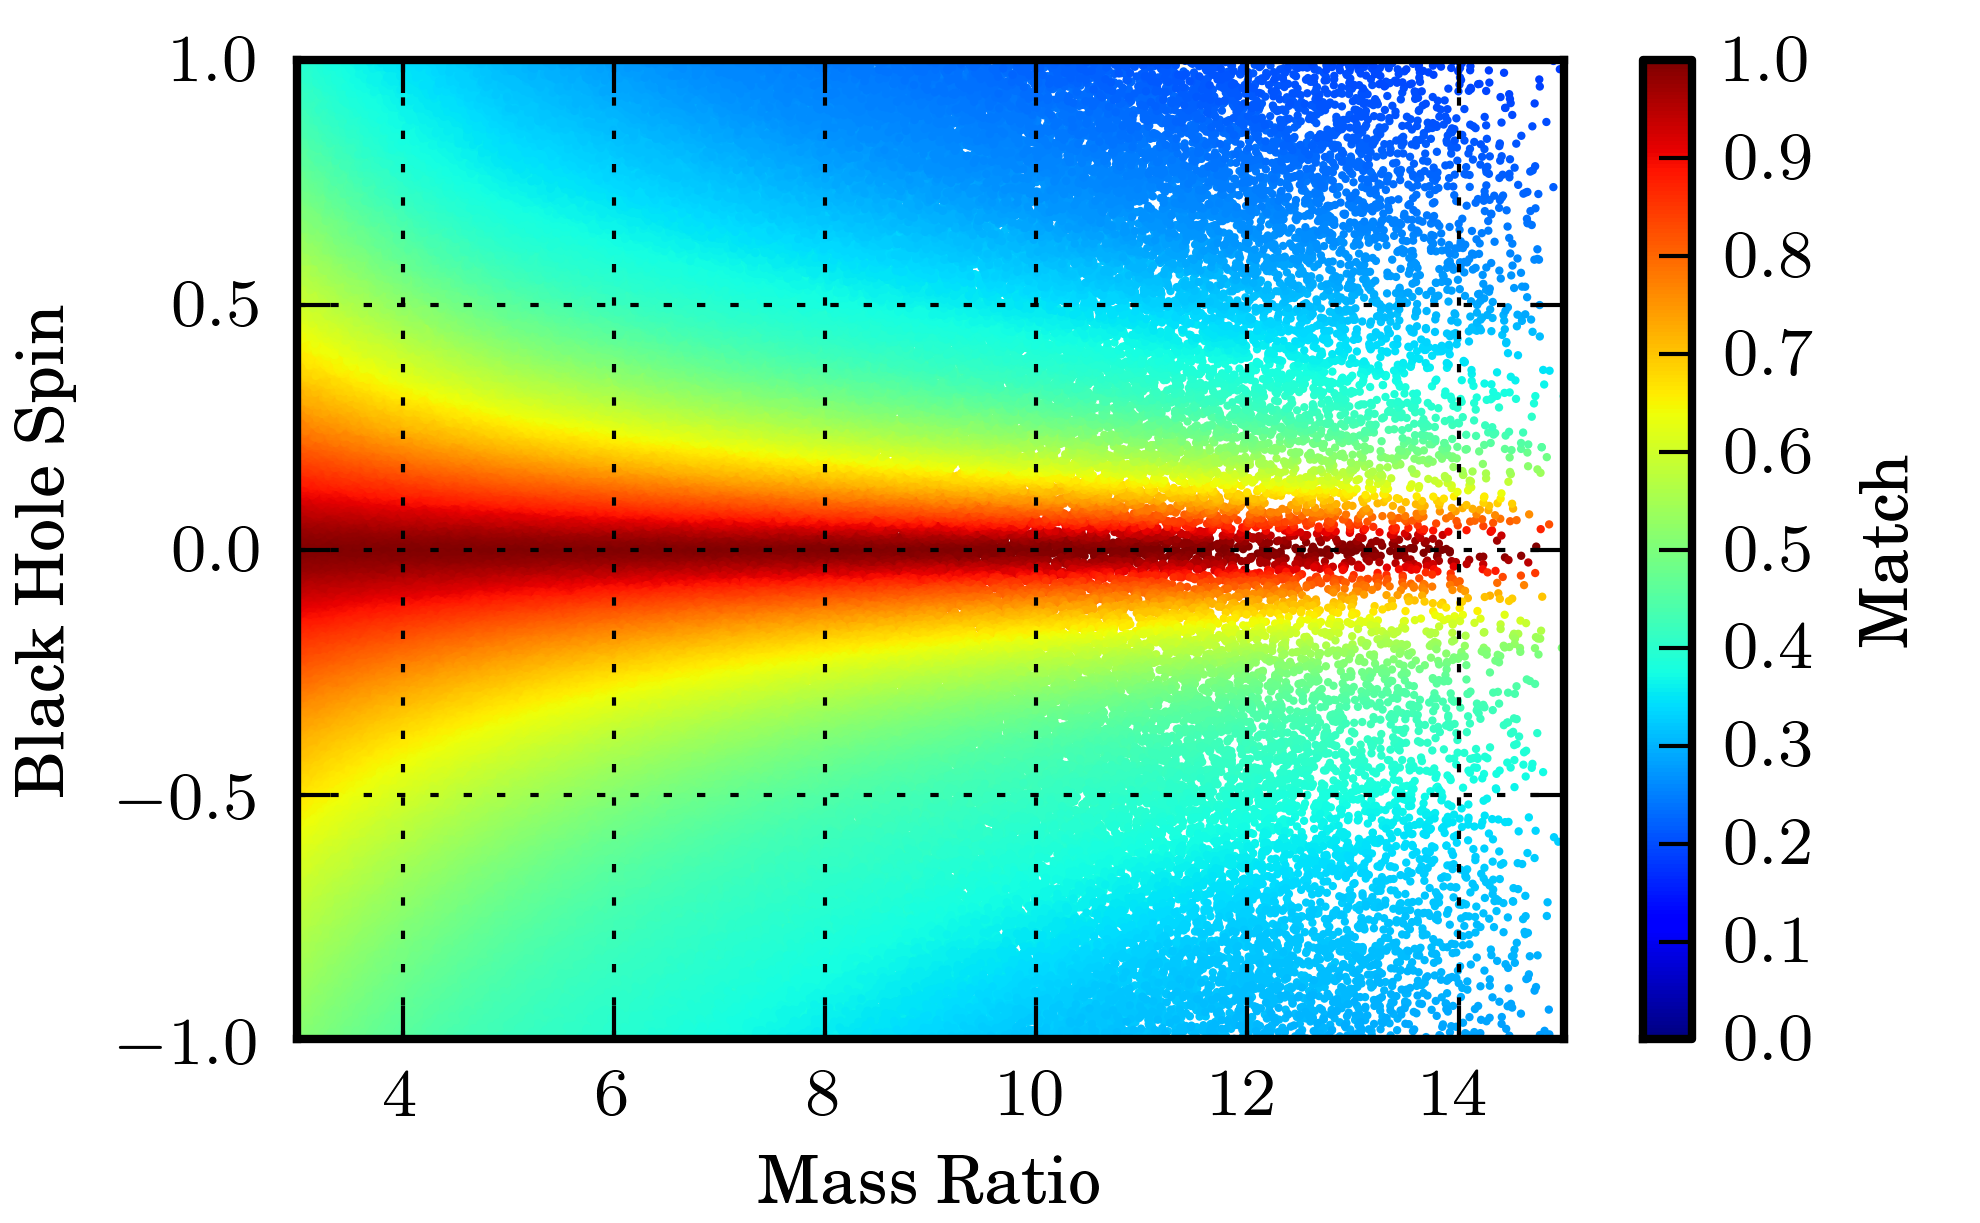
\includegraphics[width=1.0	\textwidth]{papers/nsbh_faithfulness/figure5.png}
\end{center}
\caption{\label{fig:5715t4t4}The match between TaylorT4  with 2.5\ac{PN} spin corrections
and TaylorT4 including the next-to-next-to-leading spin-orbit (3.5\ac{PN}) and spin-orbit tail 
terms (3.0\ac{PN}), as a function of the spin of the black hole
and the mass ratio of the system. Matches are calculated using the the aLIGO
zero-detuned, high-power sensitivity curve and a 15Hz lower frequency cutoff. 
In comparison to Fig.~\ref{fig:5715f2f2}, the approximant is more noticeably changed
by the additional terms. For a mass ratio of 8, the match has already 
fallen to  $ \sim 0.7 $ for $\chi \sim 0.15$. }
\end{figure}

\begin{figure*}
\begin{minipage}[l]{\columnwidth}
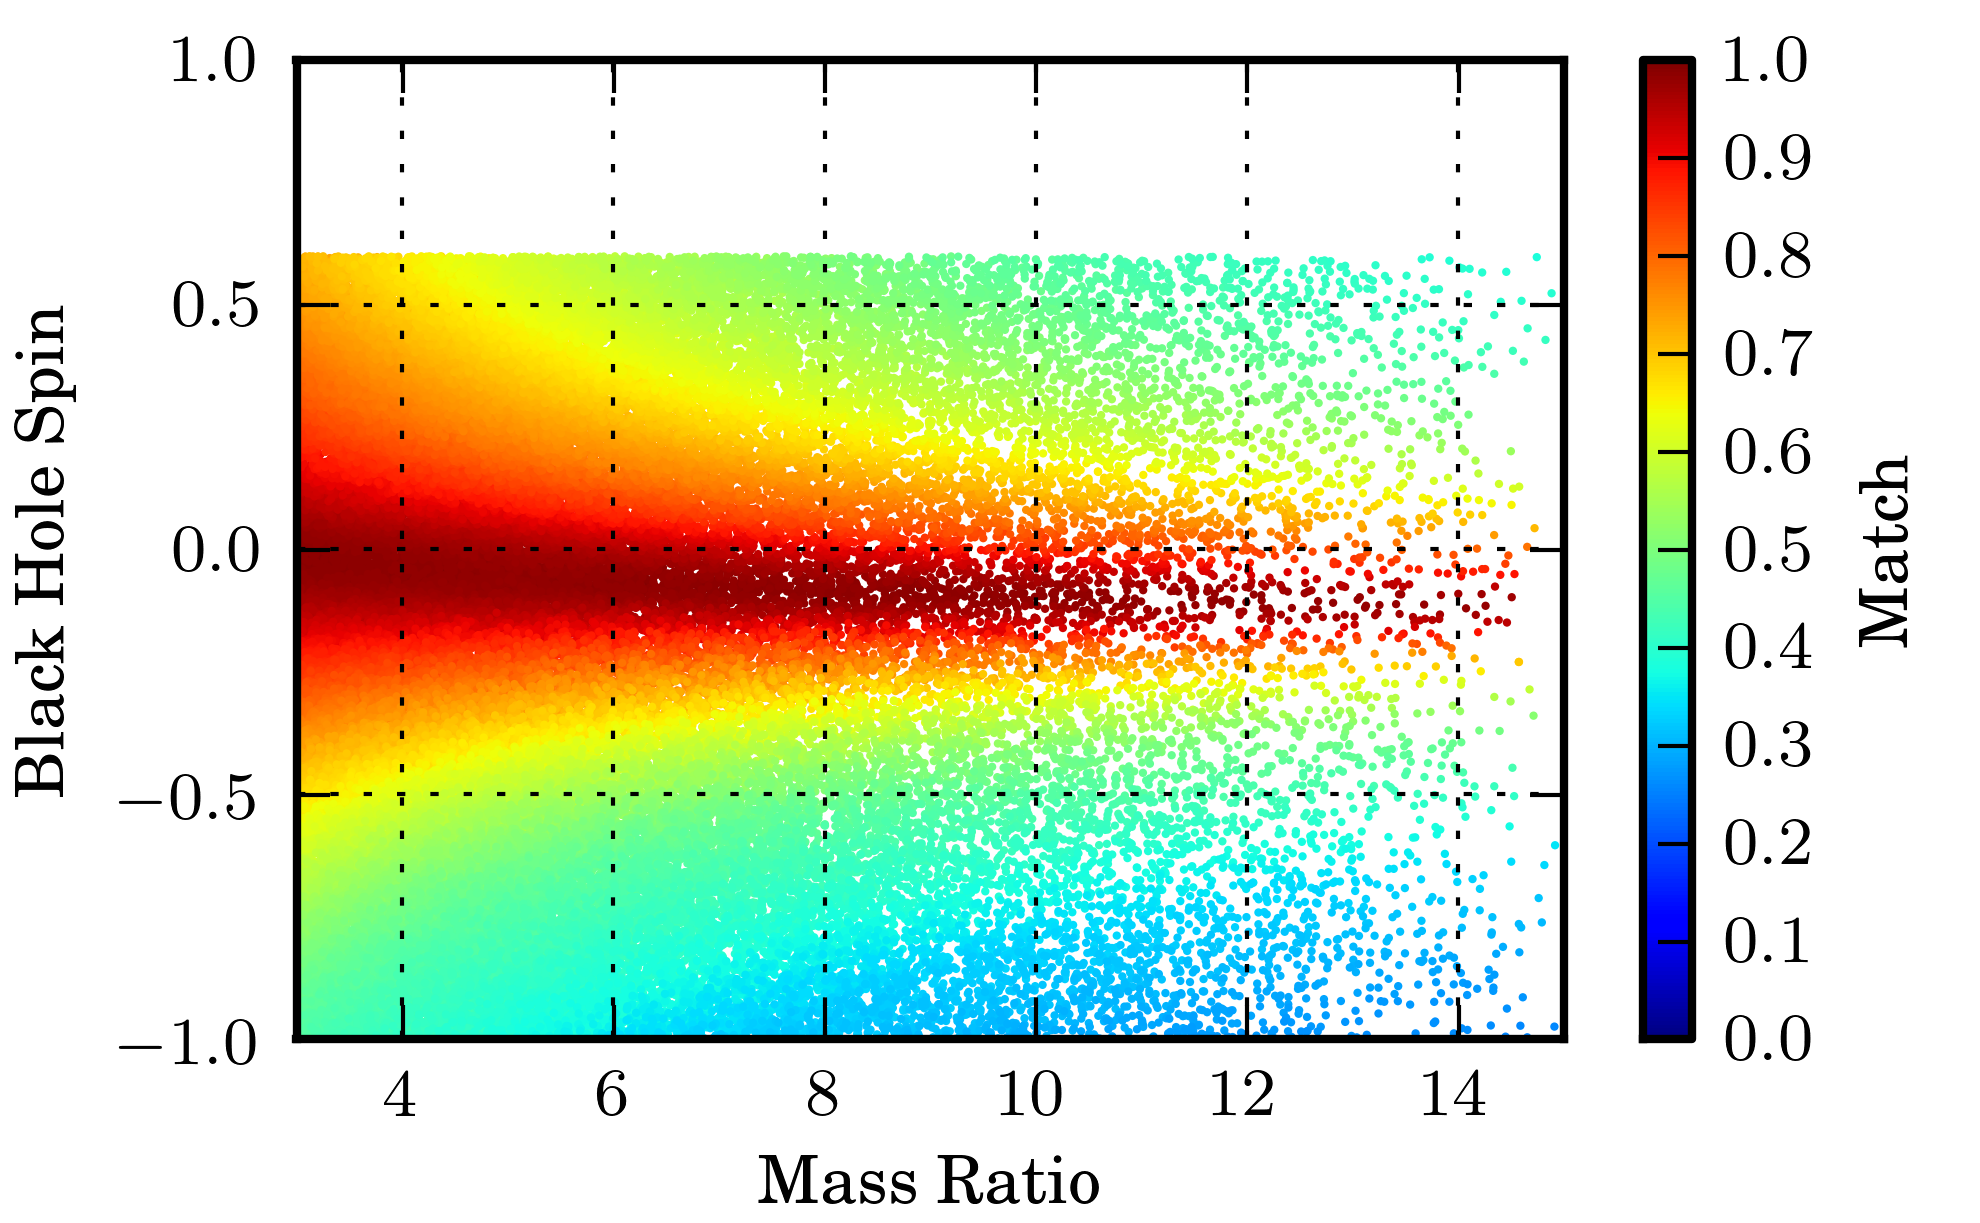
\includegraphics[width=1.0	\textwidth]{papers/nsbh_faithfulness/figure6A.png}
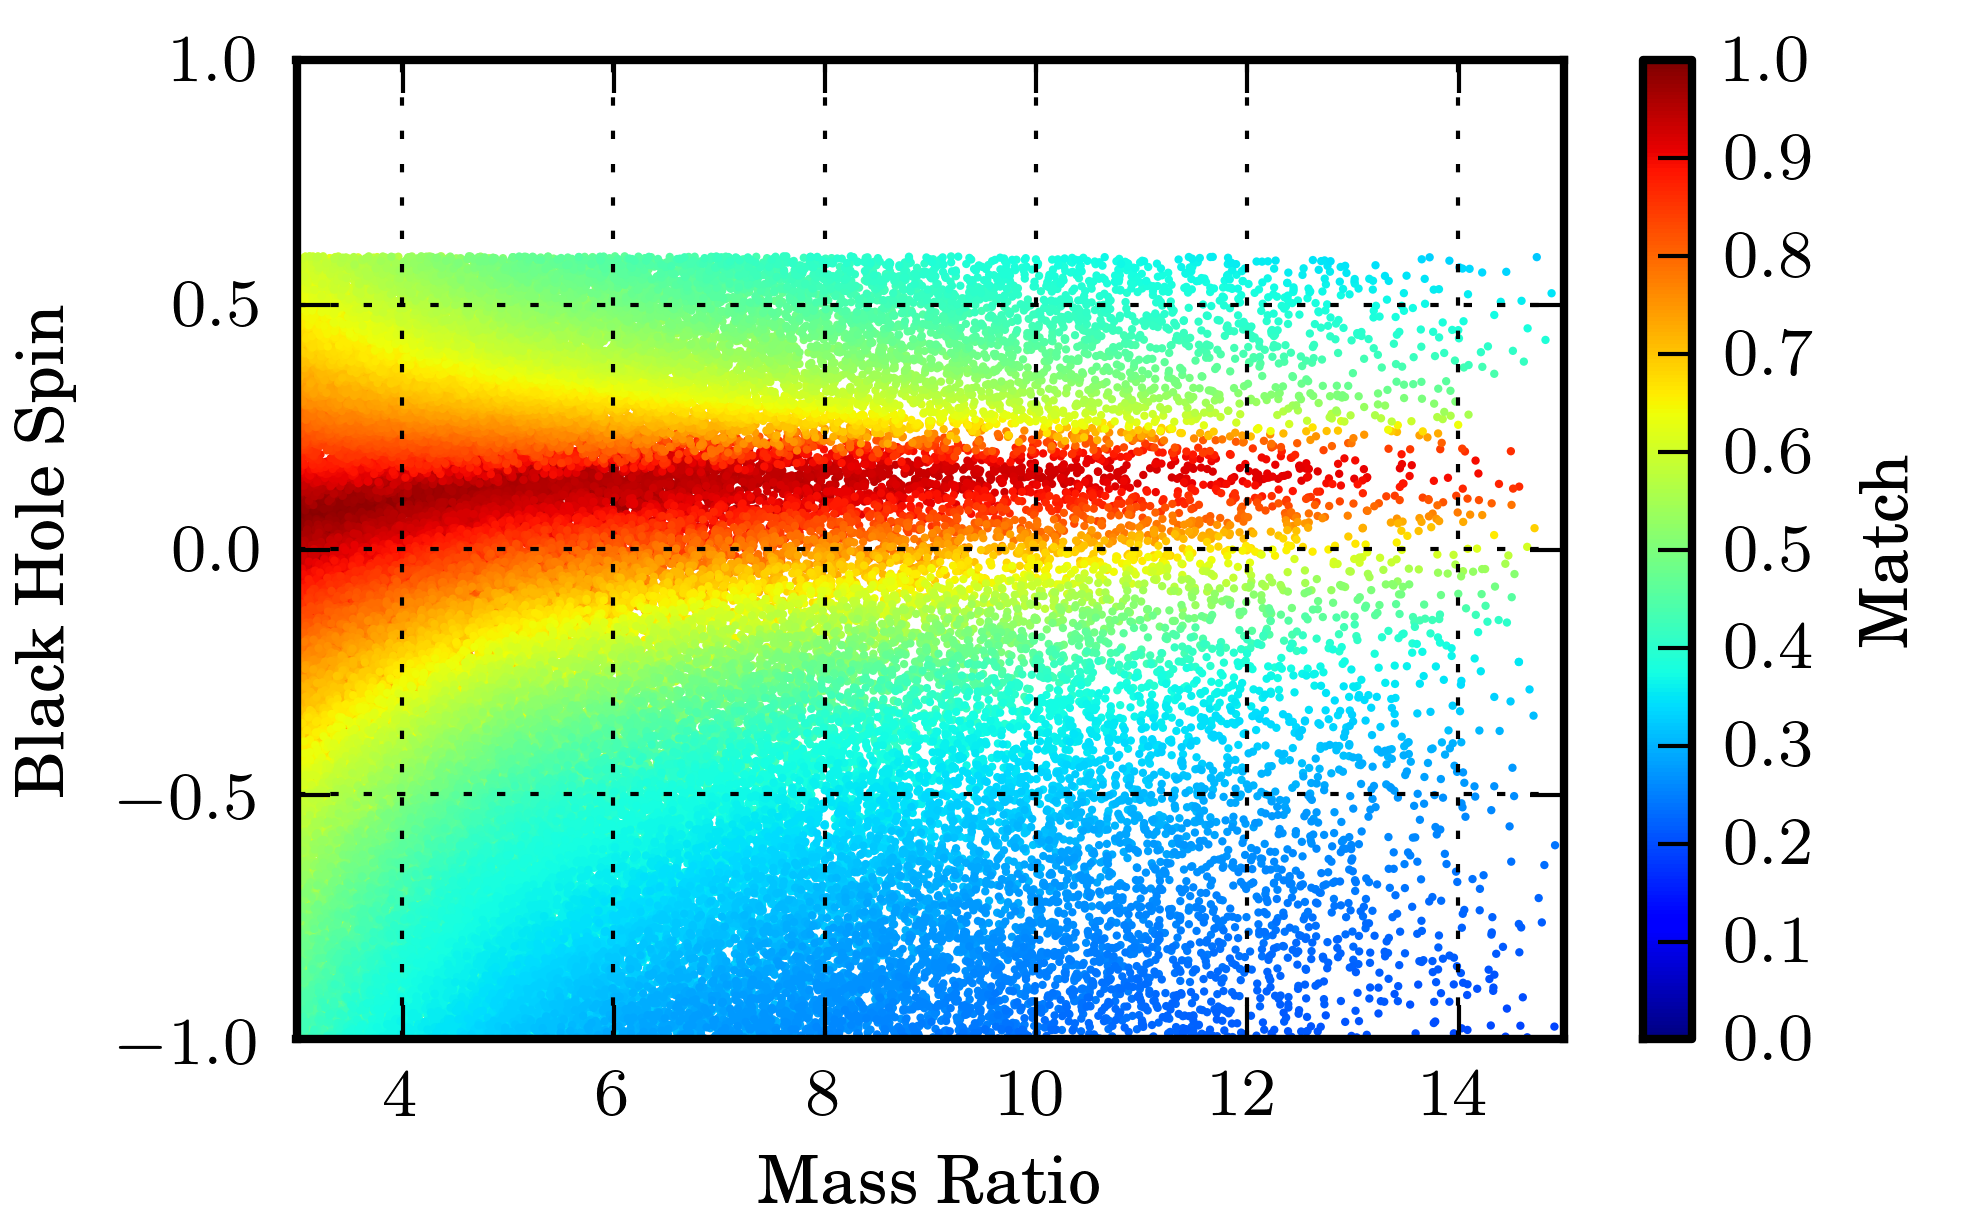
\includegraphics[width=1.0	\textwidth]{papers/nsbh_faithfulness/figure6B.png}
\caption{\label{fig:seobnrf}The match between the TaylorF2
(left) or TaylorT4 (right) and SEOBNRv1
approximants. Spin corrections for the \ac{PN} approximants are included up to 2.5\ac{PN}.
Matches are calculated using the the aLIGO zero-detuned, high-power sensitivity curve
with a 15 Hz lower frequency cutoff. As in Fig.~\ref{fig:f2f4f}, 
there is a significant reduction in match where
spin of the black hole is only moderate. Note, however, that the
\ac{PN} approximants have marginally better agreement with SEOBNRv1 than with each other.}
\end{minipage}
\end{figure*}


In Fig.~\ref{fig:seobnrf} we compare the SEOBNRv1 model to the \ac{PN} models
TaylorF2 and TaylorT4.  Since the SEOBNRv1 model is not valid
for large values of $\chi$~\cite{Taracchini:2012ig} we restrict
$\chi < 0.6$ and only report matches below this limit.  We see that,
similar to the comparison between TaylorF2 and TaylorT4, these models also have
large mismatches when the spin of the black hole is nonzero.
The large discrepancy between the waveform families indicates that higher order
\ac{PN} correction terms are required. This may also pose significant problems
for parameter estimation of \ac{NSBH} sources.



% We can perhaps argue that we are including only a few comparisons with the 3.5pN NNLO SO as 
% The 3.0 and 3.5pN spin contributions are only incompletely known. There will be additional terms,
% of as yet unkown importance due to the next SS effects, Q-M, and I think some other effects. 
% Perhaps this should be introduced earlier?



%What does sufficient mean in this context?

%%%%%%%%
\section{The TaylorR2F4 approximant}
\label{sec:R2F4}

In the previous section, we found a surprisingly large disagreement between the TaylorF2 and TaylorT4
\ac{PN} approximants when compared with waveform parameters appropriate for
\ac{NSBH} systems. We would like to distinguish how much of this is due to
differences between time domain and frequency domain approximants, and how much
of this is due to differences between the formulation of the two \ac{PN}
families.  This can easily be performed for the TaylorF2 and TaylorT2
approximants, however we need to construct an equivalent frequency domain
version of TaylorT4 to complete the comparison.

By analogy with TaylorF1 and TaylorF2~\cite{Damour:2000zb,Buonanno:2009zt},
TaylorF4 is obtained by numerically integrating the reciprocal of Eq.~\eqref{eq:t4}
in the frequency domain,
%
\begin{equation}\label{eq:f4}
%
dt/dv = 1 / A_k(v).
%
\end{equation}
%
However, this does not elucidate the differences between the TaylorT4 and
TaylorF2 approximants. Instead, we construct an analytical approximation to the
TaylorF4 approximant, which we call TaylorR2F4, by expanding Eq.~\eqref{eq:f4} in
powers of $v$. In order to make this series finite, we truncate these
additional terms at an order in $v$ higher than the order where the \ac{PN}
expansion of the energy and flux were truncated,
%
\begin{equation}
%
\frac{dt}{dv} = \left[ \frac{1}{A_{k}(v)} \right]_l = B_{k}(v) + R_{kl}(v) =
C_{kl}(v).
%
\end{equation}
%
Here $B_{k}(v)$ is the same as in the TaylorT2 approximant and $R_{kl}(v)$ are
the terms from order $v^{k+1}$ up to order $v^l$. It is important to note that
this produces a power series that is identical to the TaylorF2 approximant up
to the point where~\eqref{eq:t2} was truncated.  Thus, terms of higher order in
$v$ account for the differences between the TaylorT2 and TaylorT4 approximants.

In sec.~\ref{sec:freq_vs_time_approx} we show that TaylorR2F4 agrees well with the TaylorT4 approximant
when expanded to $v^9$ or $v^{12}$, which we shall see in the next section.  As
noted above, the second expansion in the TaylorR2F4 approximant is a different
expansion than the \ac{PN} expansion of the energy and flux.  The Fourier phase
for the TaylorR2F4 approximant can be obtained from~\eqref{eq:phaset2}  where
$B_{k}(v)$ is replaced by $C_{kl}(v)$.  This is given up to order $v^N$ as
%
\begin{equation}
%
\psi_{\mathrm{R2F4}}(f) = \psi_{F2}(f) + \sum_{i=6}^{N} \sum_{j=0}^{N}
\lambda_{i, j} f^{(i-5)/3} \log^j f,
%
\end{equation}
%
where the form of these expressions up to $N=12$ can be found in
Appendix~\ref{app:R2F4}.
Because this approximant can be analytically expressed in the frequency domain,
it can be generated relatively cheaply compared to TaylorT4. This means that it has
the potential to be used where computational efficiency and 
a higher degree of agreement with TaylorT4 is desired.
We note that the frequency-domain approximants are much faster than their
time-domain counterparts, which must integrate differential equations and perform 
a Fourier transform. Therefore, they are especially useful in computational problems 
which are waveform-generation limited, 
such as parameter estimation of signals~\cite{Aasi:2013jjl}.

%%%%%%%%
\section{Comparison of Frequency to Time Domain Approximants}
\label{sec:freq_vs_time_approx}

\begin{figure}
\begin{center}
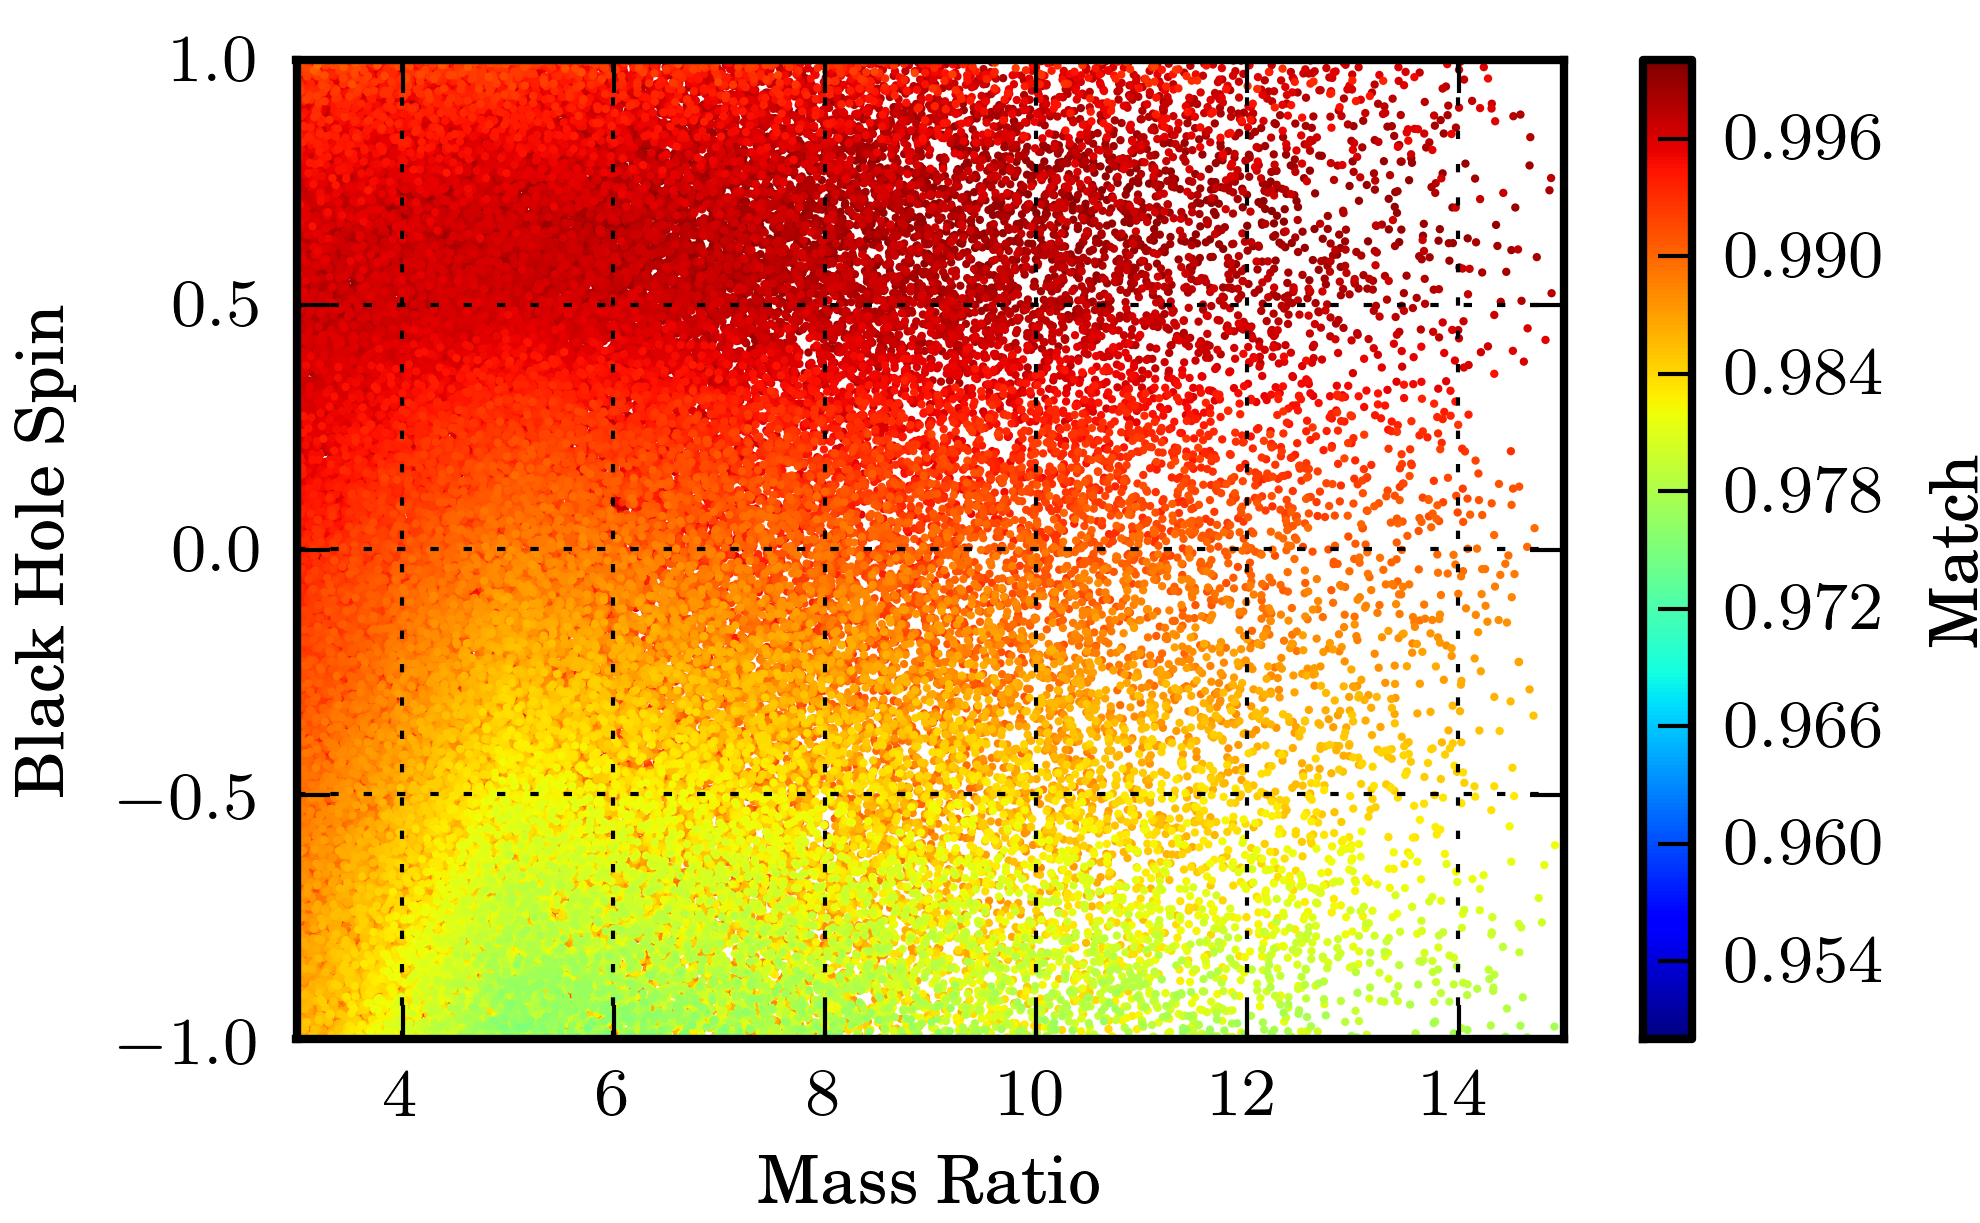
\includegraphics[width=1.0	\textwidth]{papers/nsbh_faithfulness/figure7.png}
\end{center}
\caption{\label{fig:f2t2fs} The match between TaylorF2 and TaylorT2. Both include spin 
corrections up to 2.5\ac{PN} order.
Matches are calculated using the the aLIGO
zero-detuned, high-power sensitivity curve and a 15Hz lower frequency cutoff. 
We see that the F2 and T2 approximants largely agree. The discrepancy
between the two approixmants can be reduced by expanding the frequency sweep of
the TaylorF2 approximant's amplitude to higher \ac{PN} orders. However, there
is different Gibbs phenomena between the two approximants that will cause a
discrepancy.}

\end{figure}


\begin{figure*}
\begin{minipage}[l]{\columnwidth}
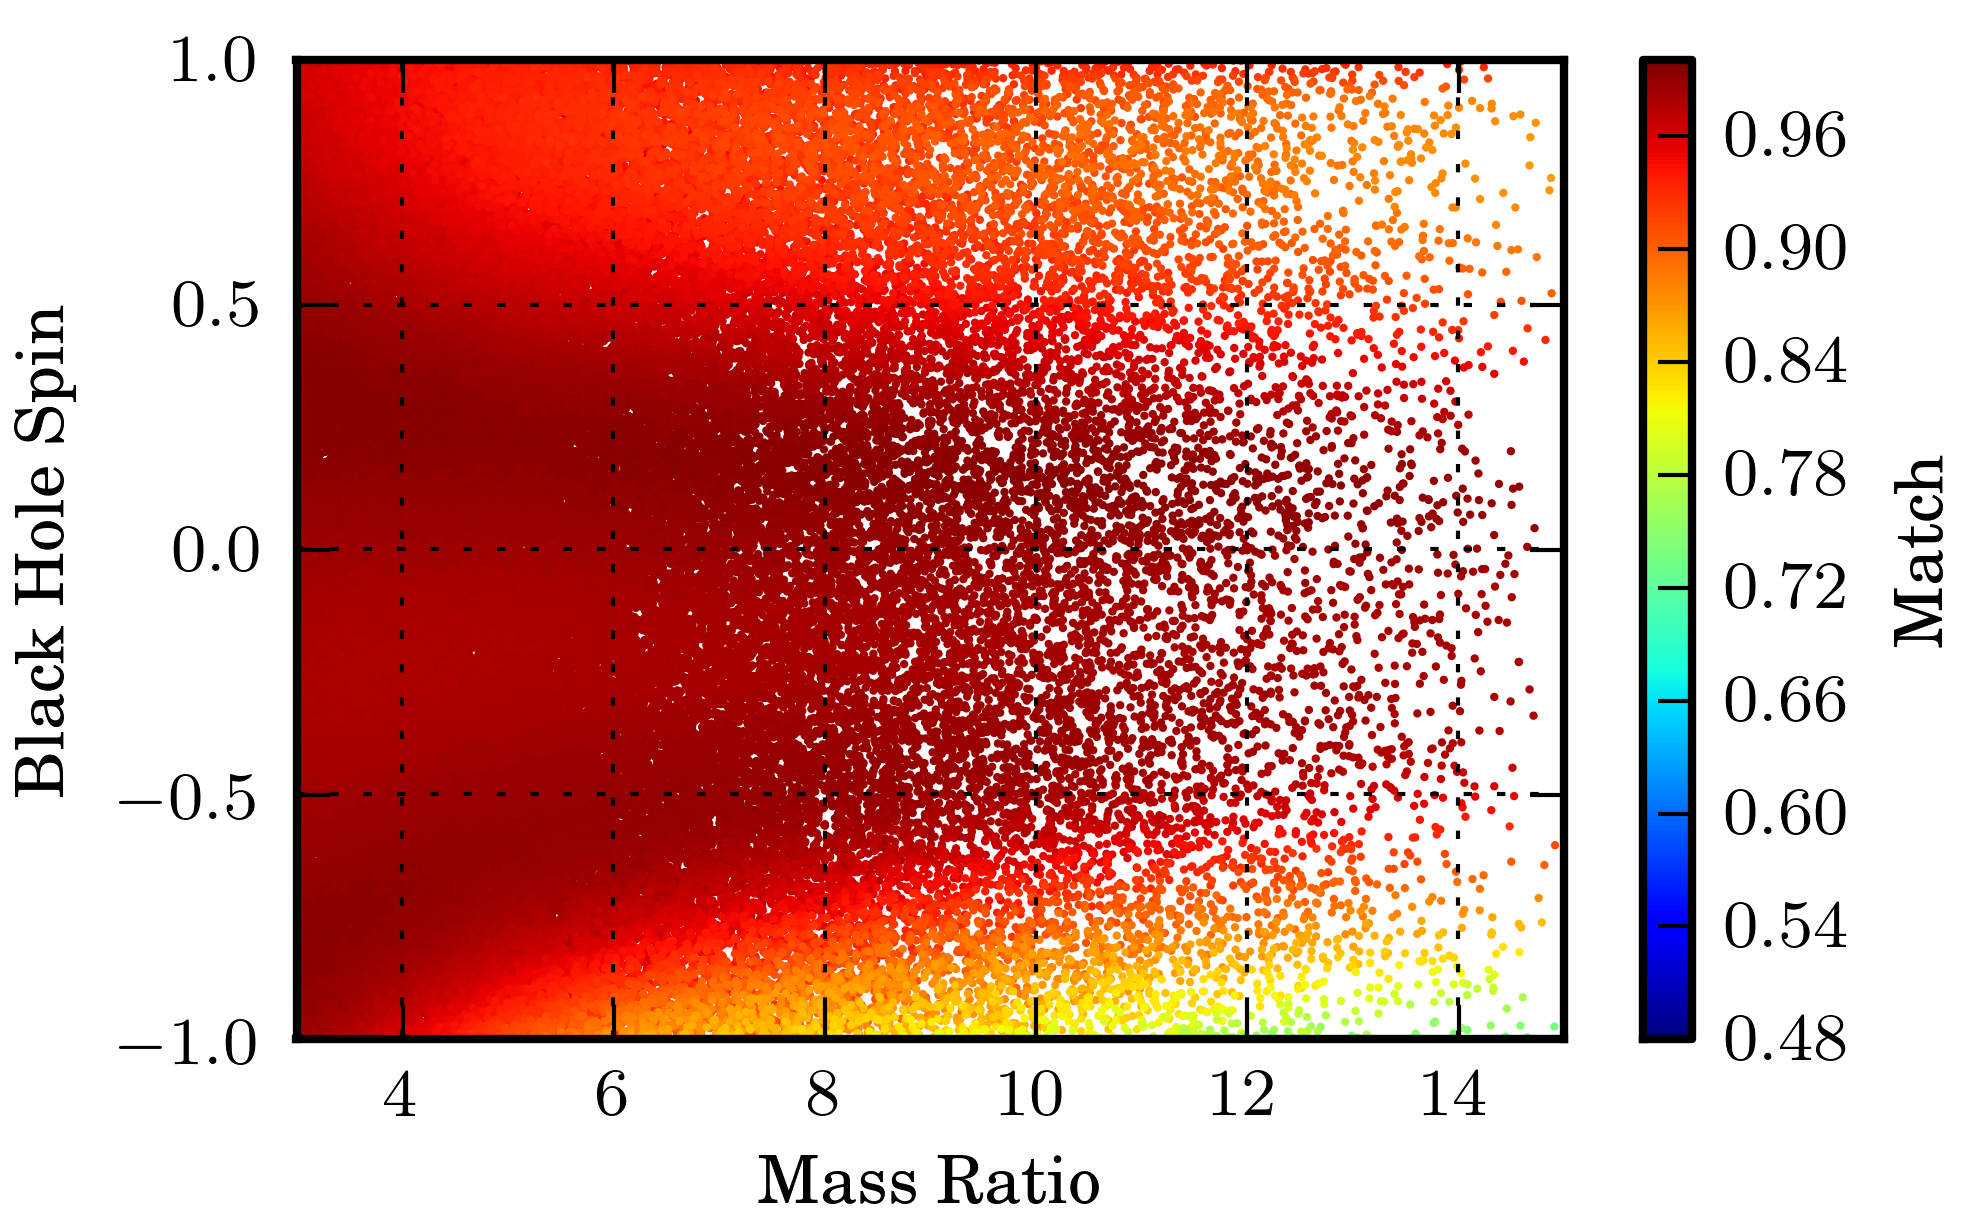
\includegraphics[width=1.0	\textwidth]{papers/nsbh_faithfulness/figure8A.png}
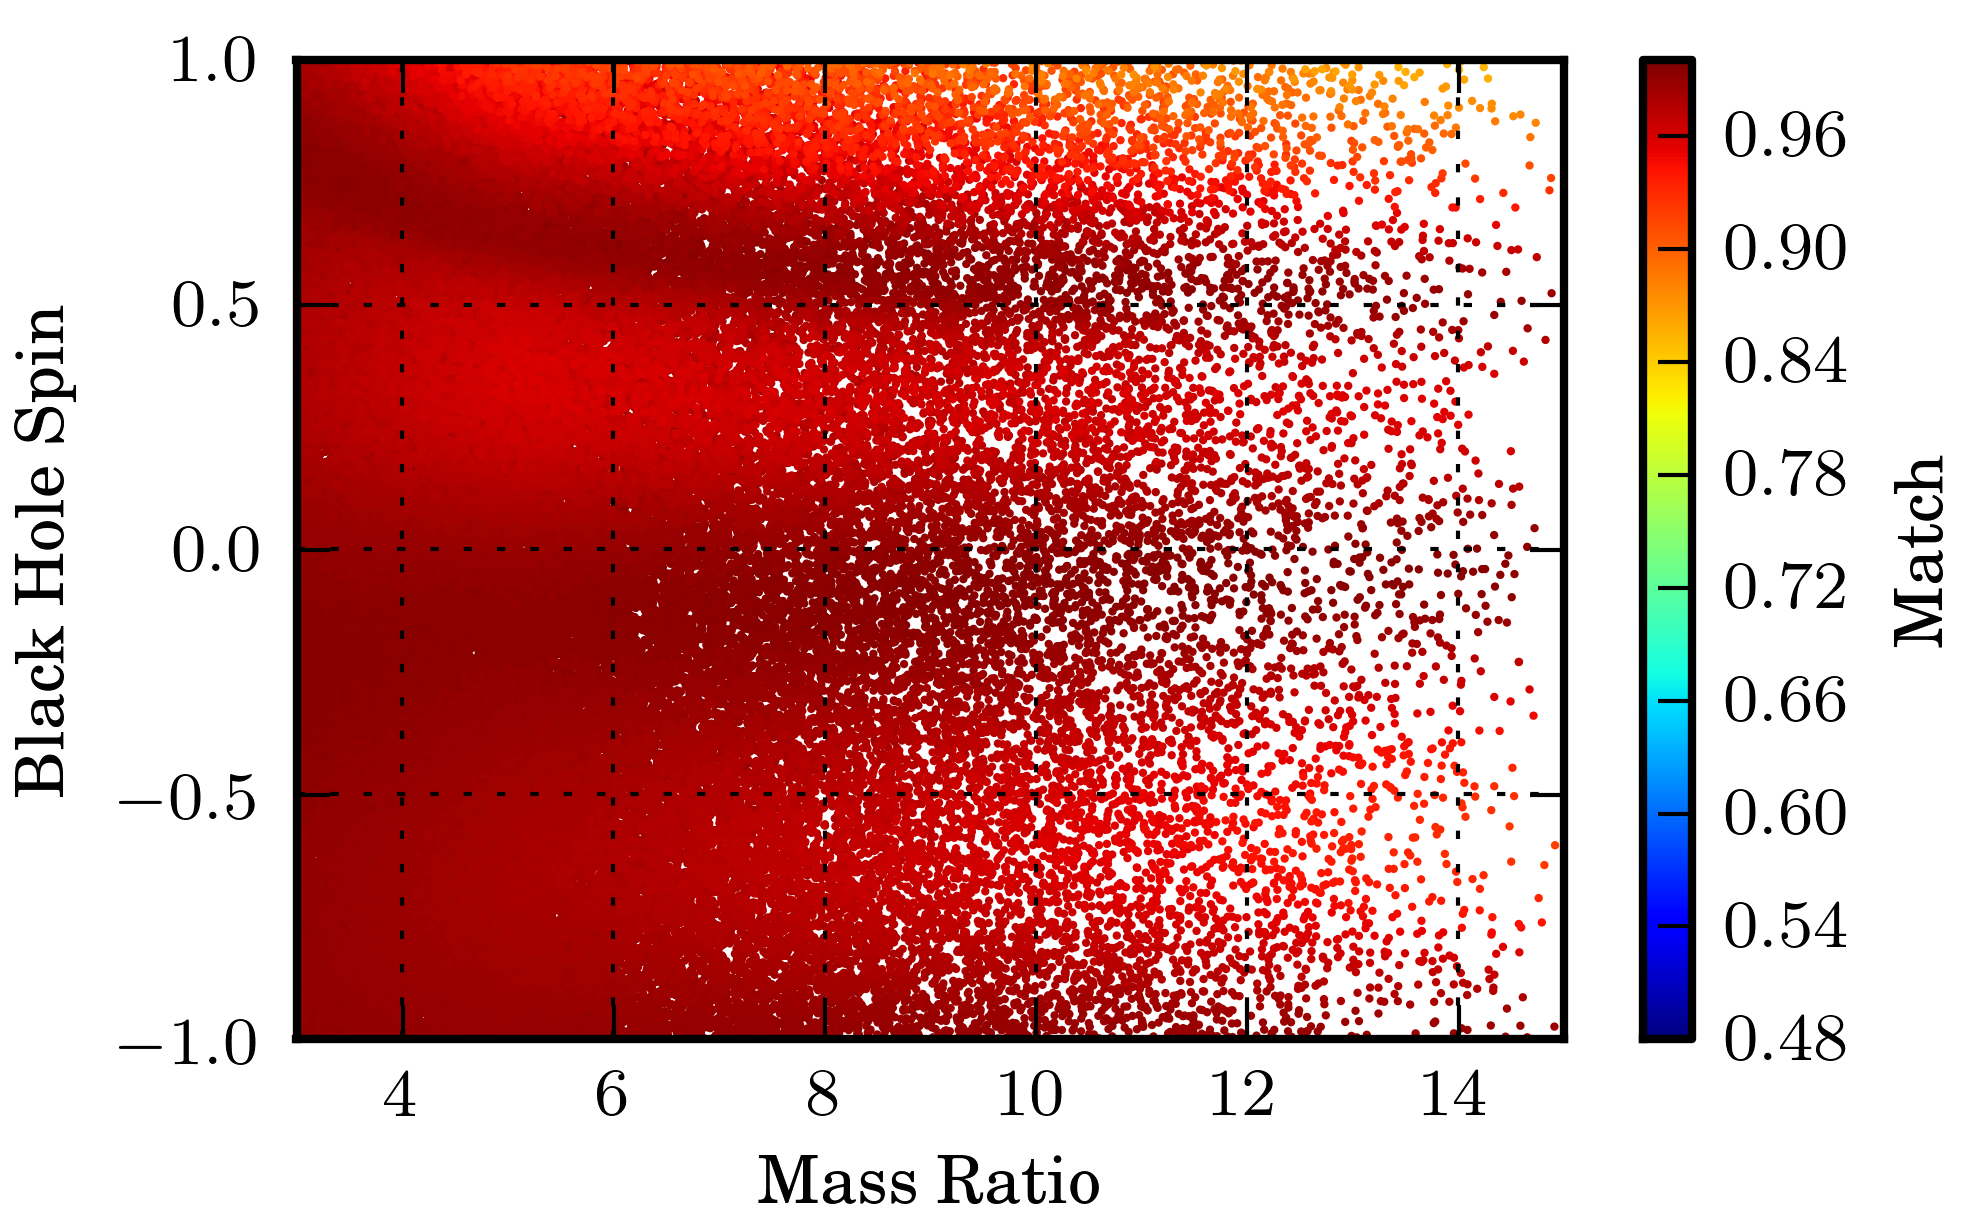
\includegraphics[width=1.0	\textwidth]{papers/nsbh_faithfulness/figure8B.png}
\caption{\label{fig:f4t4fs}The match between TaylorT4 and TaylorR2F4. Both models include
spin corrections up to 2.5 \ac{PN}. TaylorR2F4 is  re-expanded up to order $v^9$ (left) 
and $v^{12}$ (right). Matches are calculated using the the aLIGO
zero-detuned, high-power sensitivity curve and a 15Hz lower frequency cutoff. R2F4 and T4 have
high agreement over a broad range of parameters, with some visible exceptions.
Expanding up to order $v^{12}$ has generally increased
agreement with TaylorT4. }
\end{minipage}
\end{figure*}
In this section, we investigate to what extent the discrepancy between the waveform families that
was demonstrated in Sec.~\ref{sec:faithfulness} is due to the difference
between expressing approximants in the frequency and time domain alone.
We compare the new TaylorR2F4 approximant from
Sec.~\ref{sec:R2F4}, and TaylorF2, to their time domain equivalents.


We find that TaylorF2 waveforms are a good representation of
TaylorT2 waveforms, even when we consider waveforms from \ac{NSBH} systems
where the component objects are spinning. This can be seen in
Figure~\ref{fig:f2t2fs}, which shows the match between the TaylorF2 and
TaylorT2 models. In that figure, the ending frequency of both models is made to
be the same, which is accomplished by terminating the TaylorF2 waveforms at the
frequency where the generation of the equivalent TaylorT2 waveforms terminated.
We find that the TaylorF2 and TaylorT2 waveforms agree to better than $\gtrsim
95.7\%$ for the entire region investigated. For systems where the black hole
spin was positively aligned with the orbital angular momentum, the match is
$\gtrsim 97.9\%$. The discrepancy between these two models is in part due to
expanding to only Newtonian order the frequency sweep associated with the
stationary phase approximation of the TaylorF2 approximant. In addition, part
of the discrepancy results from Gibbs phenomena differences between the
approximants.
It is important to note that neither of these waveforms have termination
conditions that are determined by the physical behavior of the inspiralling
binary. The termination frequency only indicates the point at which the
approximant is certainly no longer valid. The increased match for aligned spin
waveforms is due to the higher frequency cutoff, which pushes the termination
frequency out of the most sensitive part of the zero-detuned, high-power aLIGO
sensitivity curve.

Figure~\ref{fig:f4t4fs} shows a comparison between the TaylorR2F4 and TaylorT4
models. In that figure, the second expansion associated with the TaylorR2F4
model is extended to order $v^{9}$ (left) and $v^{12}$ (right), and the ending frequency of both
is that corresponding to the \ac{MECO}.  We show that the TaylorR2F4 model is
adequate for a large range of parameters as a computationally inexpensive
substitute for TaylorT4. 

Since the mismatch between the TaylorF2 and TaylorT4 models is not due to
differences between the time domain and frequency domain approximants, this
indicates that the effective higher order \ac{PN} terms used in the
construction of TaylorR2F4, which are also intrinsically present in TaylorT4,
are still significant. To obtain better agreement between the
different \ac{PN} approximants we consider, it is necessary to extend the
\ac{PN} expansions of the energy and flux equations to include 
unknown higher order terms, particularly ones that involve 
the spin of the objects. 

%%%%%%%%
\section{Accumulation of Phase Discrepancy}
\label{sec:faithfulness_phase}

\begin{figure*}
\begin{center}
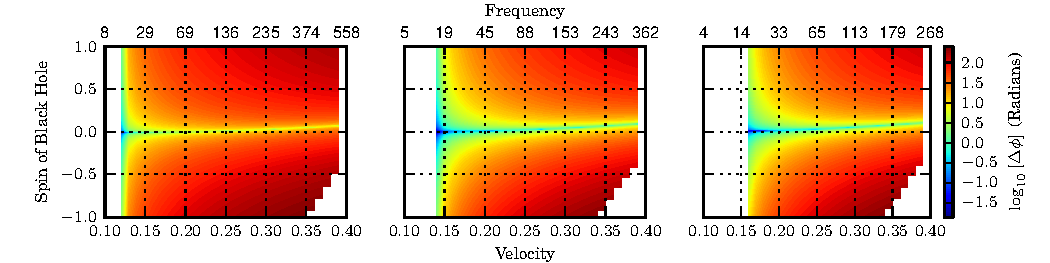
\includegraphics[]{papers/nsbh_faithfulness/figure9.pdf}
\end{center}
\caption{\label{fig:T2T4pa} The accumulation of phase differences between
TaylorT2 and TaylorT4, for systems with component masses $(m_1, m_2)$ of
$(1.4\Msun, 6\Msun)$ (left), $(1.4\Msun, 10\Msun)$ (center), and $(1.4\Msun,
14\Msun)$ (right). The approximants include spin terms up to 2.5\ac{PN}.
The calculation starts from the velocity corresponding to a
 gravitational-wave  frequency of $15$Hz, continues to the velocity on the horizontal axis,
and reports the difference in accumulated gravitational-wave phase between the waveforms. The feature
in the bottom right corner of each plot arises because the TaylorT2 approximant is no longer monotonic.
Note that large phase differences accumulate at very low velocities $v \sim 0.2 $
for even small black hole spins.}

\end{figure*}

\begin{figure*}
\begin{center}
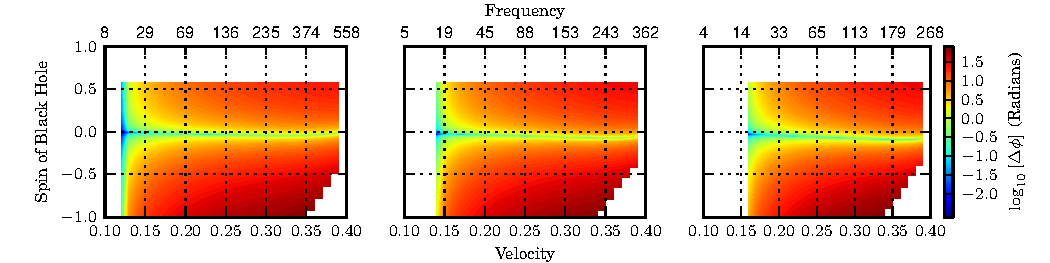
\includegraphics[]{papers/nsbh_faithfulness/figure10.pdf}
\end{center}
\caption{\label{fig:T2SEpa} The accumulation of phase difference between
TaylorT2 and SEOBNRv1, for systems with component masses $(m_1, m_2)$ of
$(6\Msun, 1.4\Msun)$ (left), $(10\Msun, 1.4\Msun)$ (center), and $(14\Msun,
1.4\Msun)$ (right). TaylorT2 includes spin terms up to 2.5\ac{PN}.
The calculation starts from the velocity corresponding to a gravitational-wave  frequency of $15$Hz, 
continues to the velocity on the horizontal axis,
and reports the difference in accumulated gravitational-wave phase between the waveforms. The feature
in the bottom right corner of each plot arises because the TaylorT2 approximant is no longer monotonic.
As in Fig.~\ref{fig:T2T4pa}, a large phase difference is
accumulated at low velocities and small black hole spins.}

\end{figure*}


In the previous sections, we demonstrated that the two \ac{PN} approximants,
TaylorF2 and TaylorT4, and the SEOBNRv1 model are not faithful to each other.
We also showed that this is not due to the differences between frequency and
time domain waveforms.  From the construction of the TaylorR2F4 approximant, we
also demonstrated that the two \ac{PN} families can be written in a way that is
consistent up to the chosen \ac{PN} order, but where TaylorR2F4 contains higher
order in $v$ corrections that account for the differences between the models.
Since these are higher order corrections, they should start to become important
to the orbital phasing only at high velocities, and thus high  gravitational-wave 
frequencies. In this section we investigate where, for systems with parameters
corresponding to \ac{NSBH} binaries, the approximants diverge. We do this by
examining the accumulation of phase as a function of orbital velocity and
reporting the difference in the number of  gravitational-wave  cycles between different
approximants.

In Fig.~\ref{fig:T2T4pa}, we examine the difference in the accumulated phase
between TaylorT2 and TaylorT4 for three example systems with component masses
$(m_1, m_2)$ of $(6\Msun, 1.4\Msun)$, $(10\Msun, 1.4\Msun)$, and $(14\Msun,
1.4\Msun)$. We see that the phase difference between the two models quickly
grows to tens of radians, even when the black hole spin magnitude is small.
This is also true when comparing TaylorT2 and SEOBNRv1, as can be seen in
Fig.~\ref{fig:T2SEpa}.  In the latter case, there is also a noticeable
deviation away from the line of zero spin where for unknown reasons the two
models diverge and subsequently converge.

%%%%%%%%
\section{Accumulation of mismatch}
\label{sec:faithfulness_match_accumulation}

\begin{figure*}
\begin{center}
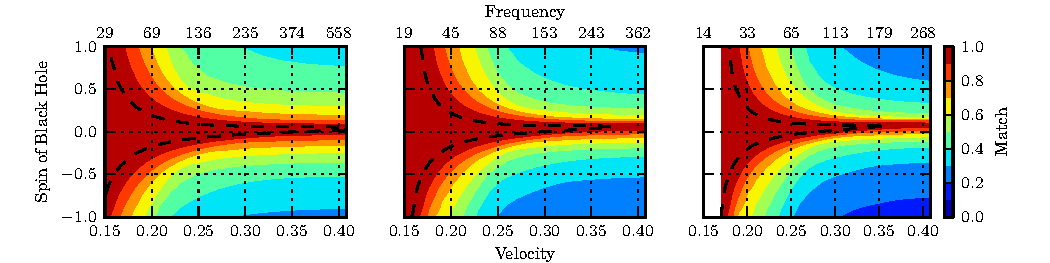
\includegraphics[]{papers/nsbh_faithfulness/figure11.pdf}
\end{center}
\caption{\label{fig:F2T4ma} The match between TaylorF2 and TaylorT4
integrated from 15 Hz up to the designated frequency for systems with component
masses $(m_1, m_2)$ of $(1.4\Msun, 6\Msun)$ (left), $(1.4\Msun, 10\Msun)$
(center), and $(1.4\Msun, 14\Msun)$ (right).  Both approximants include spin corrections up to 2.5\ac{PN}.
Matches are calculated using the the aLIGO
zero-detuned, high-power sensitivity curve. A contour at a match of 0.97 is
indicated by the dotted line.  The match follows the general features seen in
the phase difference comparison of Fig.~\ref{fig:T2T4pa} and drops
significantly, even at relatively low velocities. For the $(1.4\Msun, 6\Msun)$ system with a black
hole spin $\chi = 0.5 $, the match has already dropped to $\sim 0.5$ at a velocity of only $\sim 0.25$.
}
\end{figure*}


\begin{figure*}
\begin{center}
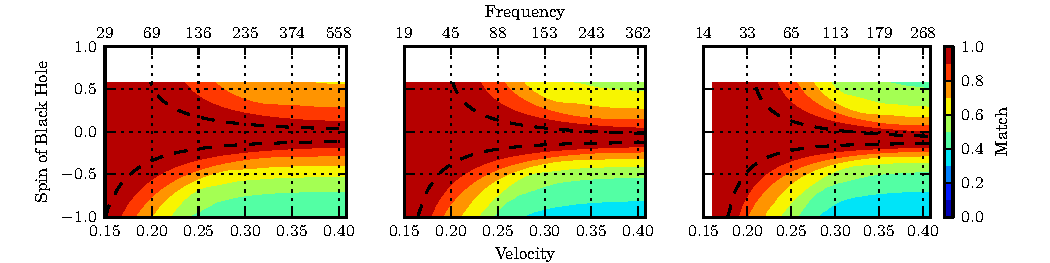
\includegraphics[]{papers/nsbh_faithfulness/figure12.pdf}
\end{center}
\caption{\label{fig:F2SEma} The match between the TaylorF2 and SEOBNRv1 models
integrated from 15 Hz up to the designated frequency for systems with component
masses $(m_1, m_2)$ of $(6\Msun, 1.4\Msun)$ (left), $(10\Msun, 1.4\Msun)$
(center), and $(14\Msun, 1.4\Msun)$ (right). TaylorF2 includes spin corrections up to 2.5\ac{PN}.
Matches are calculated using the the aLIGO
zero-detuned, high-power sensitivity curve. A contour at a match of 0.97 is
indicated by the dotted line. We note that, although the match is marginally
improved compared to Fig.~\ref{fig:F2T4ma}, there are still large
disagreements at velocities as low as 0.25.}

\end{figure*}


As  gravitational-wave  detectors are not directly sensitive to phase differences alone, it
is useful to compute how the match, which incorporates the sensitivity of a
 gravitational-wave  detector, changes as a function of the upper frequency cutoff used for
the calculation. In this section we demonstrate at which frequencies and
corresponding velocities the match between waveform families drops. To do so,
we define an inner product between waveforms that is a function of the upper
frequency cutoff. This inner product is then used in the match calculation of
Eq.~\eqref{eq:match}.

In Fig.~\ref{fig:F2T4ma}, we examine the match between TaylorF2 and TaylorT4,
integrated from a lower frequency cutoff of 15 Hz up to the upper frequency
cutoff indicated on the horizontal axis. This is compared for the same three
example systems as in Sec.~\ref{sec:faithfulness_phase}. The match is shown
across the range of allowable values of the black hole spin and the neutron
star spin is set to zero. We see that the match drops precipitously even at low
velocities and relatively modest spin magnitudes. For example, for a system
with $m_1=6\Msun$, $m_2=1.4\Msun$, and a dimensionless spin of 0.5 for the
black hole, the match drops below 0.7 at a velocity of only 0.23. The loss in
match is more pronounced with increasing mass ratio. 

In Fig.~\ref{fig:F2SEma}, we examine the match between TaylorF2 and SEOBNRv1,
integrated from a lower frequency cutoff of 15Hz up to the upper frequency
cutoff indicated on the horizontal axis. Again, the match drops for large spin
magnitudes at relatively low velocities, although, just as the TaylorF2
approximant has shown better matches with the SEOBNRv1 approximant than with
the TaylorT4 approximant, this occurs at somewhat higher velocities. This shows
clearly that significant portions of the loss in match seen in
Sec.~\ref{sec:faithfulness} occurs at unexpectedly low velocities.


\section{Detection searches and Early aLIGO}
\label{sec:effectualness_and_flow}

In the previous sections, we have demonstrated a substantial loss in match between
different \ac{PN} and EOB models of \ac{NSBH} binaries. These discrepancies
will cause substantial biases in attempts to measure the parameters of
detected systems with aLIGO. However, when detecting systems the
\emph{fitting factor}, rather than the match, is the quantity that is used to
assess the effectualness of a search~\cite{Apostolatos:1996rf}. The fitting
factor maximizes the match between a signal and a bank of templates designed
to capture e.g. $97\%$ of the optimal signal-to-noise ratio. The template bank is constructed to be 
valid for the same range of masses and spins used
throughout this chapter and detailed in Sec~\ref{sec:introduction}. Discrepancies in
match due to differing approximants may be compensated for by allowing a waveform
to match to a template with shifted parameters.
Figs.~\ref{fig:spin2q} and~\ref{fig:spin2q7} show the fitting
factor of a TaylorF2 aligned spin template bank when used to detect TaylorT4
waveforms. Fig.~\ref{fig:spin2q} shows the distribution of fittings factors for approximants that include up to the 2.5\ac{PN} 
spin corrections. Fig.~\ref{fig:spin2q7} demonstrates the effect of adding the higher order
3.0\ac{PN} spin-orbit tail and 3.5\ac{PN} spin-orbit corrections.
Construction of these aligned spin banks use the method introduced
in Ref.~\cite{Brown:2012qf} and is described in more detail in Ref.~\cite{Harry:2013tca}.
There is substantial improvement in the fitting factors of aligned spin systems when
adding the higher order spin corrections, but no improvement for anti-aligned spin systems. 
Although the loss in fitting factor is not as significant as the loss in match shown in
Figs.~\ref{fig:f2f4f} and~\ref{fig:f2t4fso}, aLIGO \ac{NSBH} searches will isncur a substantial loss in 
signal-to-noise ratio for anti-aligned spins, if the accuracy of \ac{NSBH} waveforms is not improved. 

\begin{figure}
\begin{center}
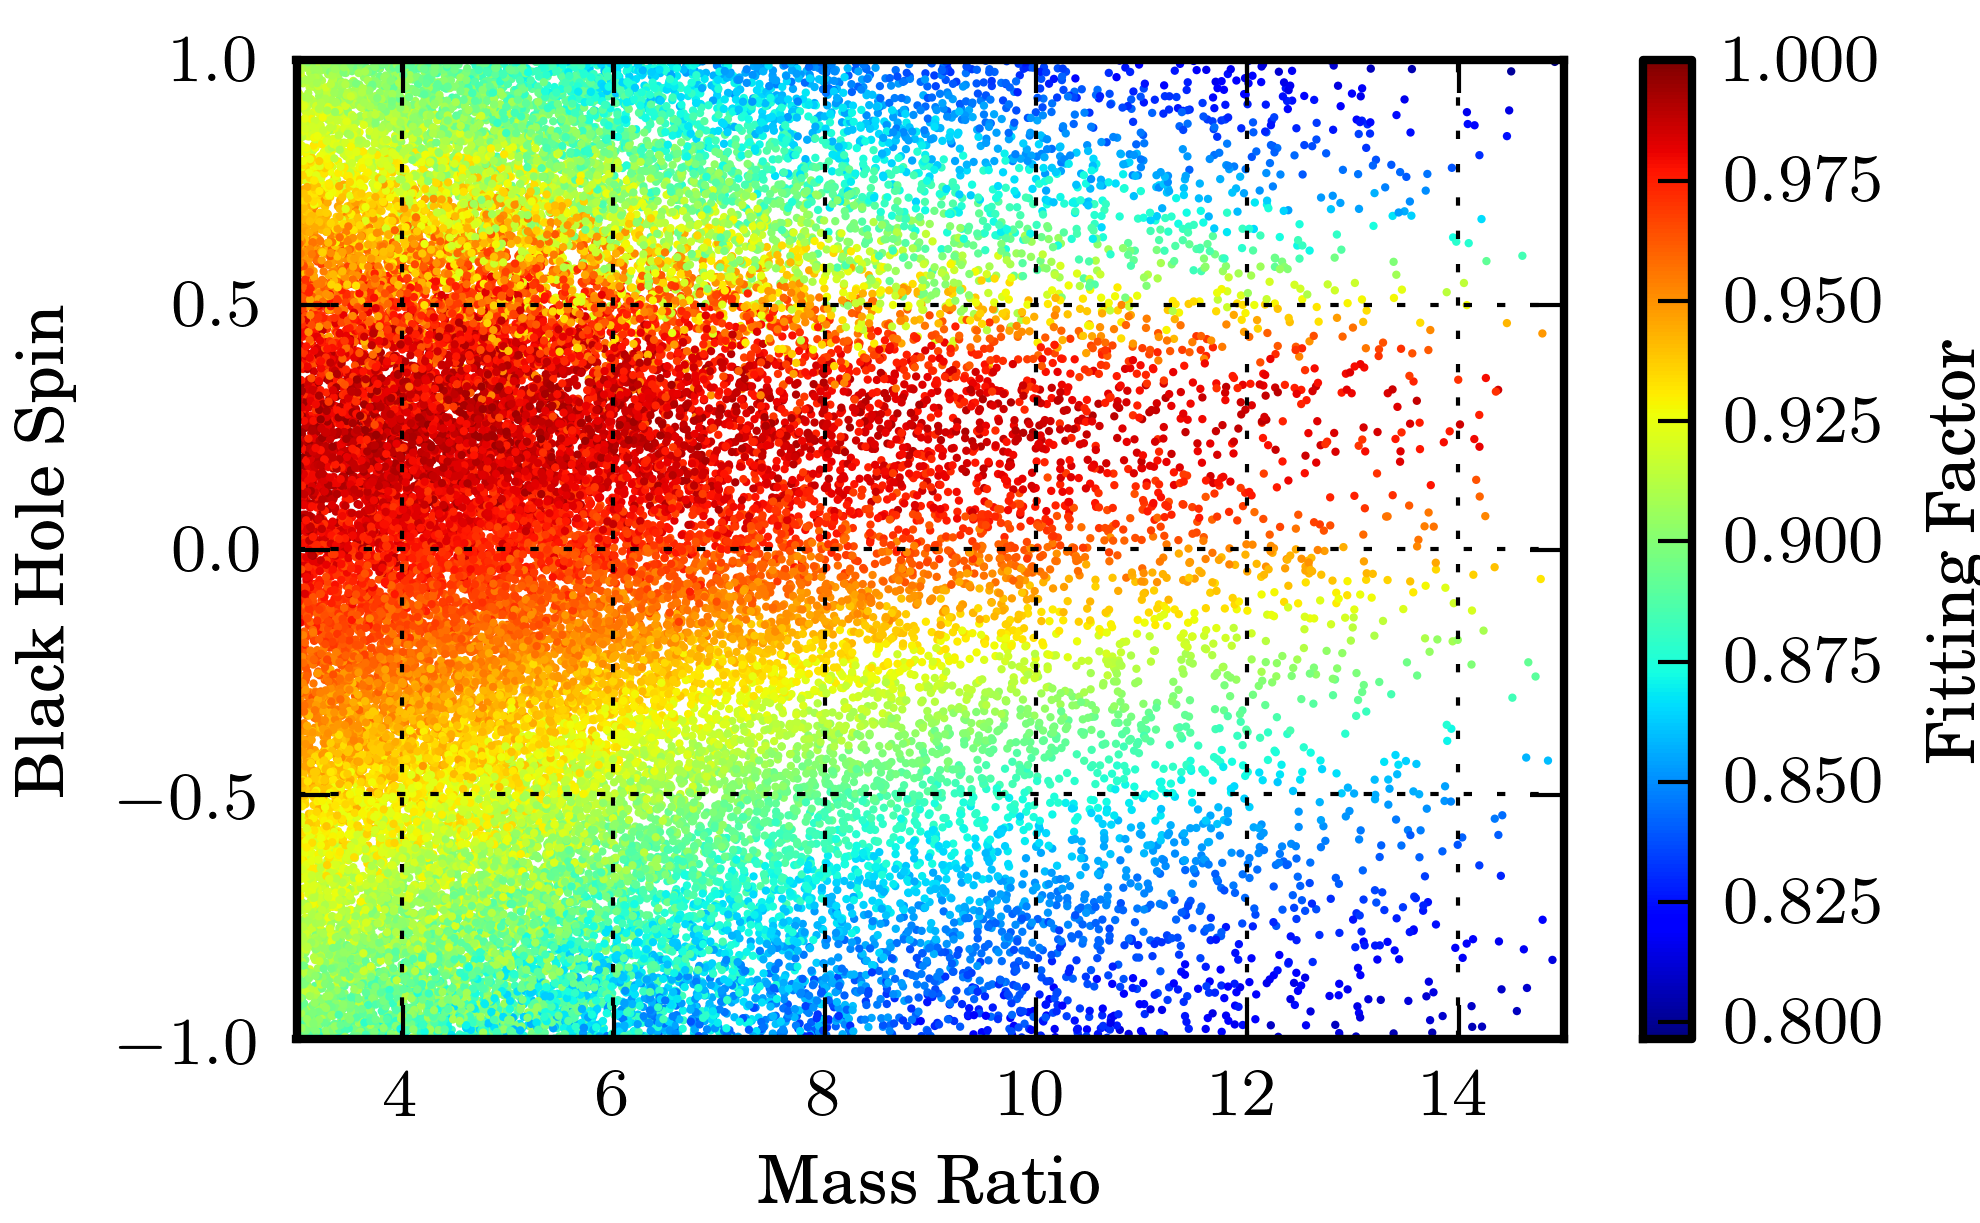
\includegraphics[width=1.0	\textwidth]{papers/nsbh_faithfulness/figure13.png}
\end{center}
\caption{\label{fig:spin2q}The fitting factor between the TaylorF2 and
TaylorT4 approximants as a function of the spin of the black hole
and the mass ratio of the system, when maximizing the match over a bank of
TaylorF2 waveforms. All approximants include spin corrections up to 2.5\ac{PN}.
Matches are calculated using the the aLIGO
zero-detuned, high-power sensitivity curve and a 15Hz lower frequency cutoff. In 
comparison to the match of these approximants shown in Fig.~\ref{fig:f2f4f}, we see that
while allowing for the maximization over a bank of templates has improved the overall agreement, 
it is unable to entirely make up for the poor match. 
}
\end{figure}

\begin{figure}
\begin{center}
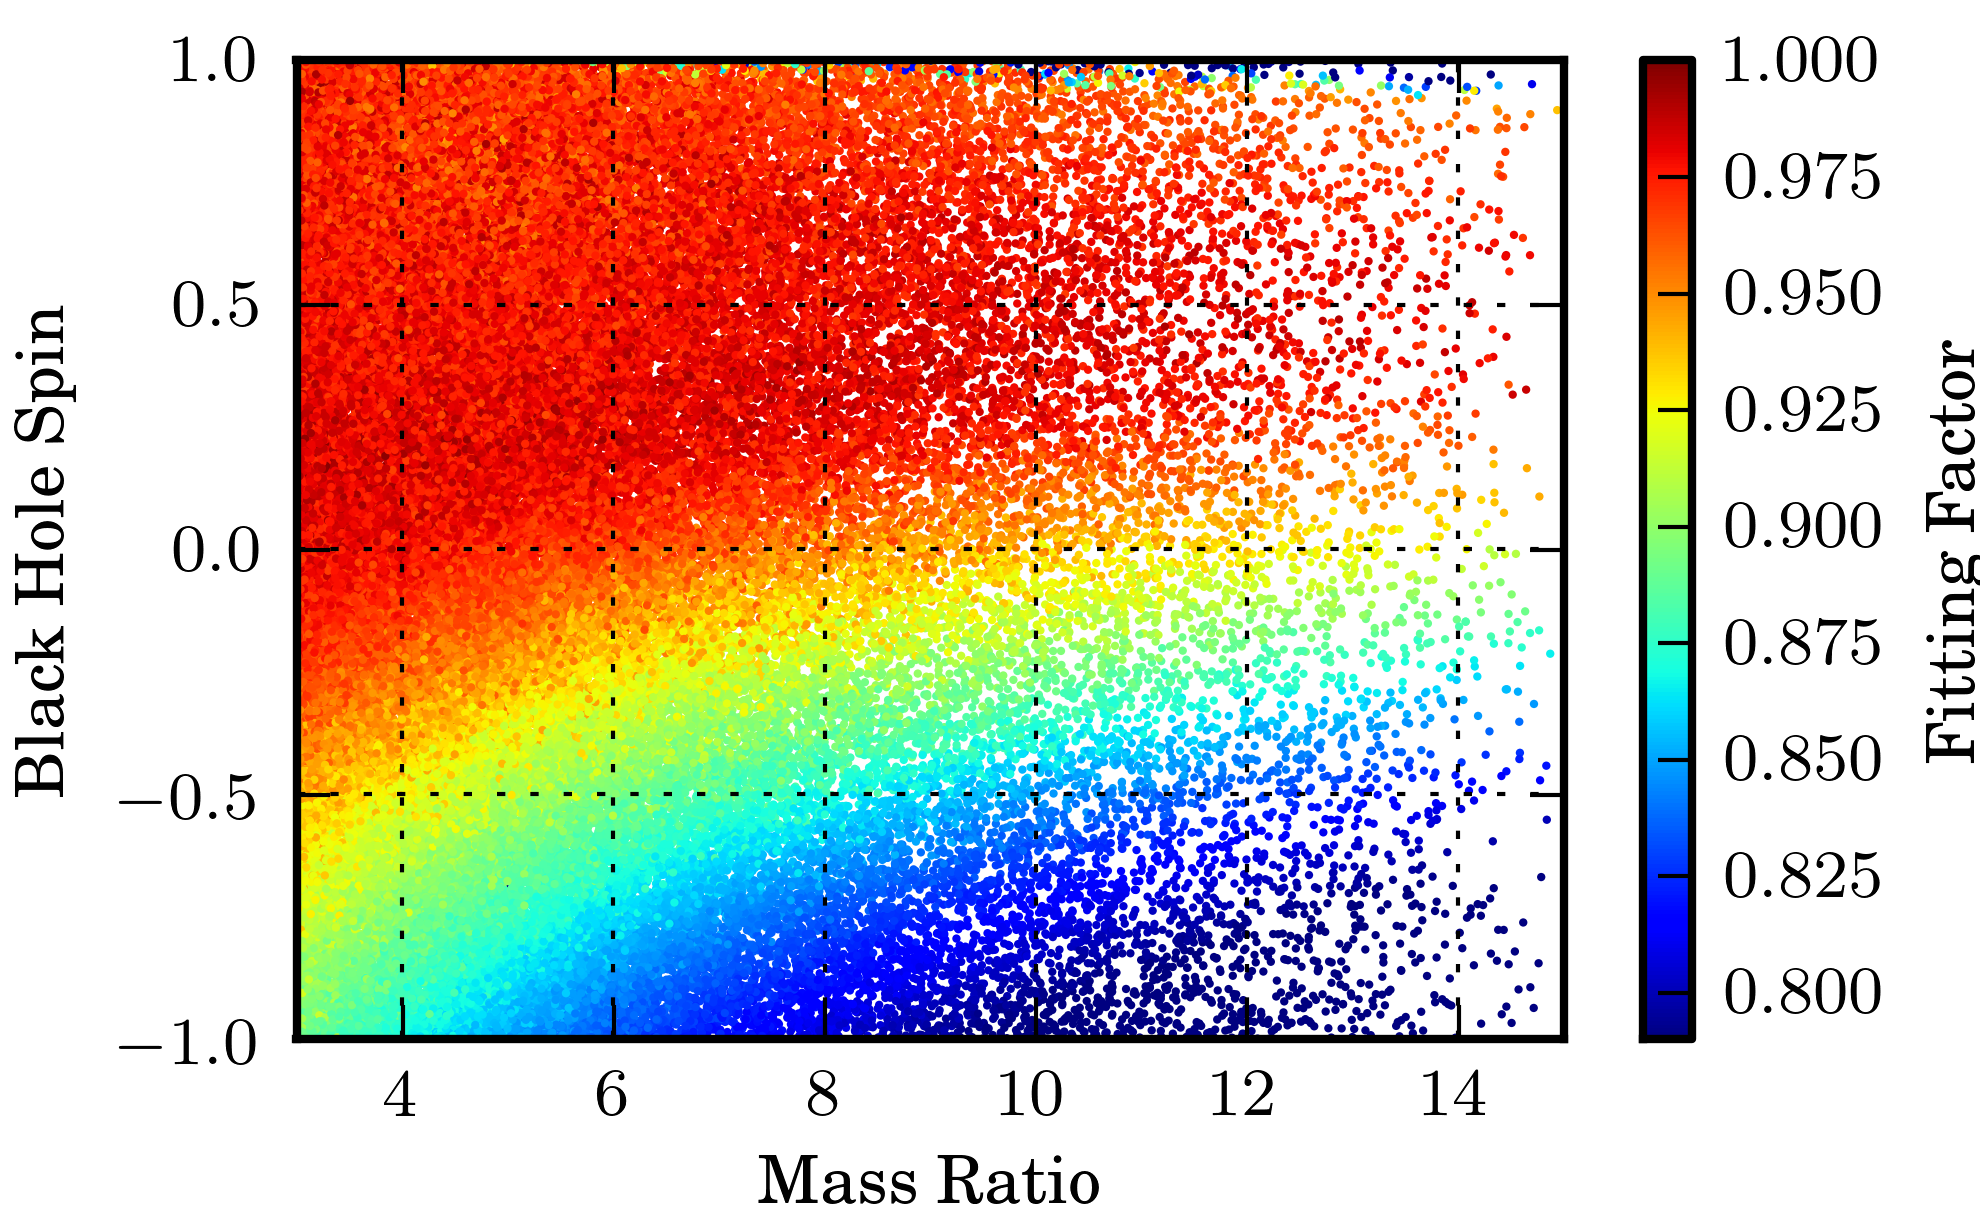
\includegraphics[width=1.0	\textwidth]{papers/nsbh_faithfulness/figure14.png}
\end{center}
\caption{\label{fig:spin2q7}The fitting factor between the TaylorF2 and
TaylorT4 approximants as a function of the spin of the black hole
and the mass ratio of the system, when maximizing the match over a bank of
TaylorF2 waveforms. All approximants include the 3.5\ac{PN} spin-orbit and 3.0\ac{PN} 
spin-orbit tail corrections. 
Matches are calculated using the the aLIGO
zero-detuned, high-power sensitivity curve and a 15Hz lower frequency cutoff. In 
comparison to the fitting factors shown in Fig.~\ref{fig:spin2q}, we see that adding
the higher order spin corrections has resulted in substantially improved fitting factors for 
systems where the spin is aligned with the orbital angular momentum. There is no 
improvement for anti-aligned systems.
}
\end{figure}


\begin{figure}
\begin{center}
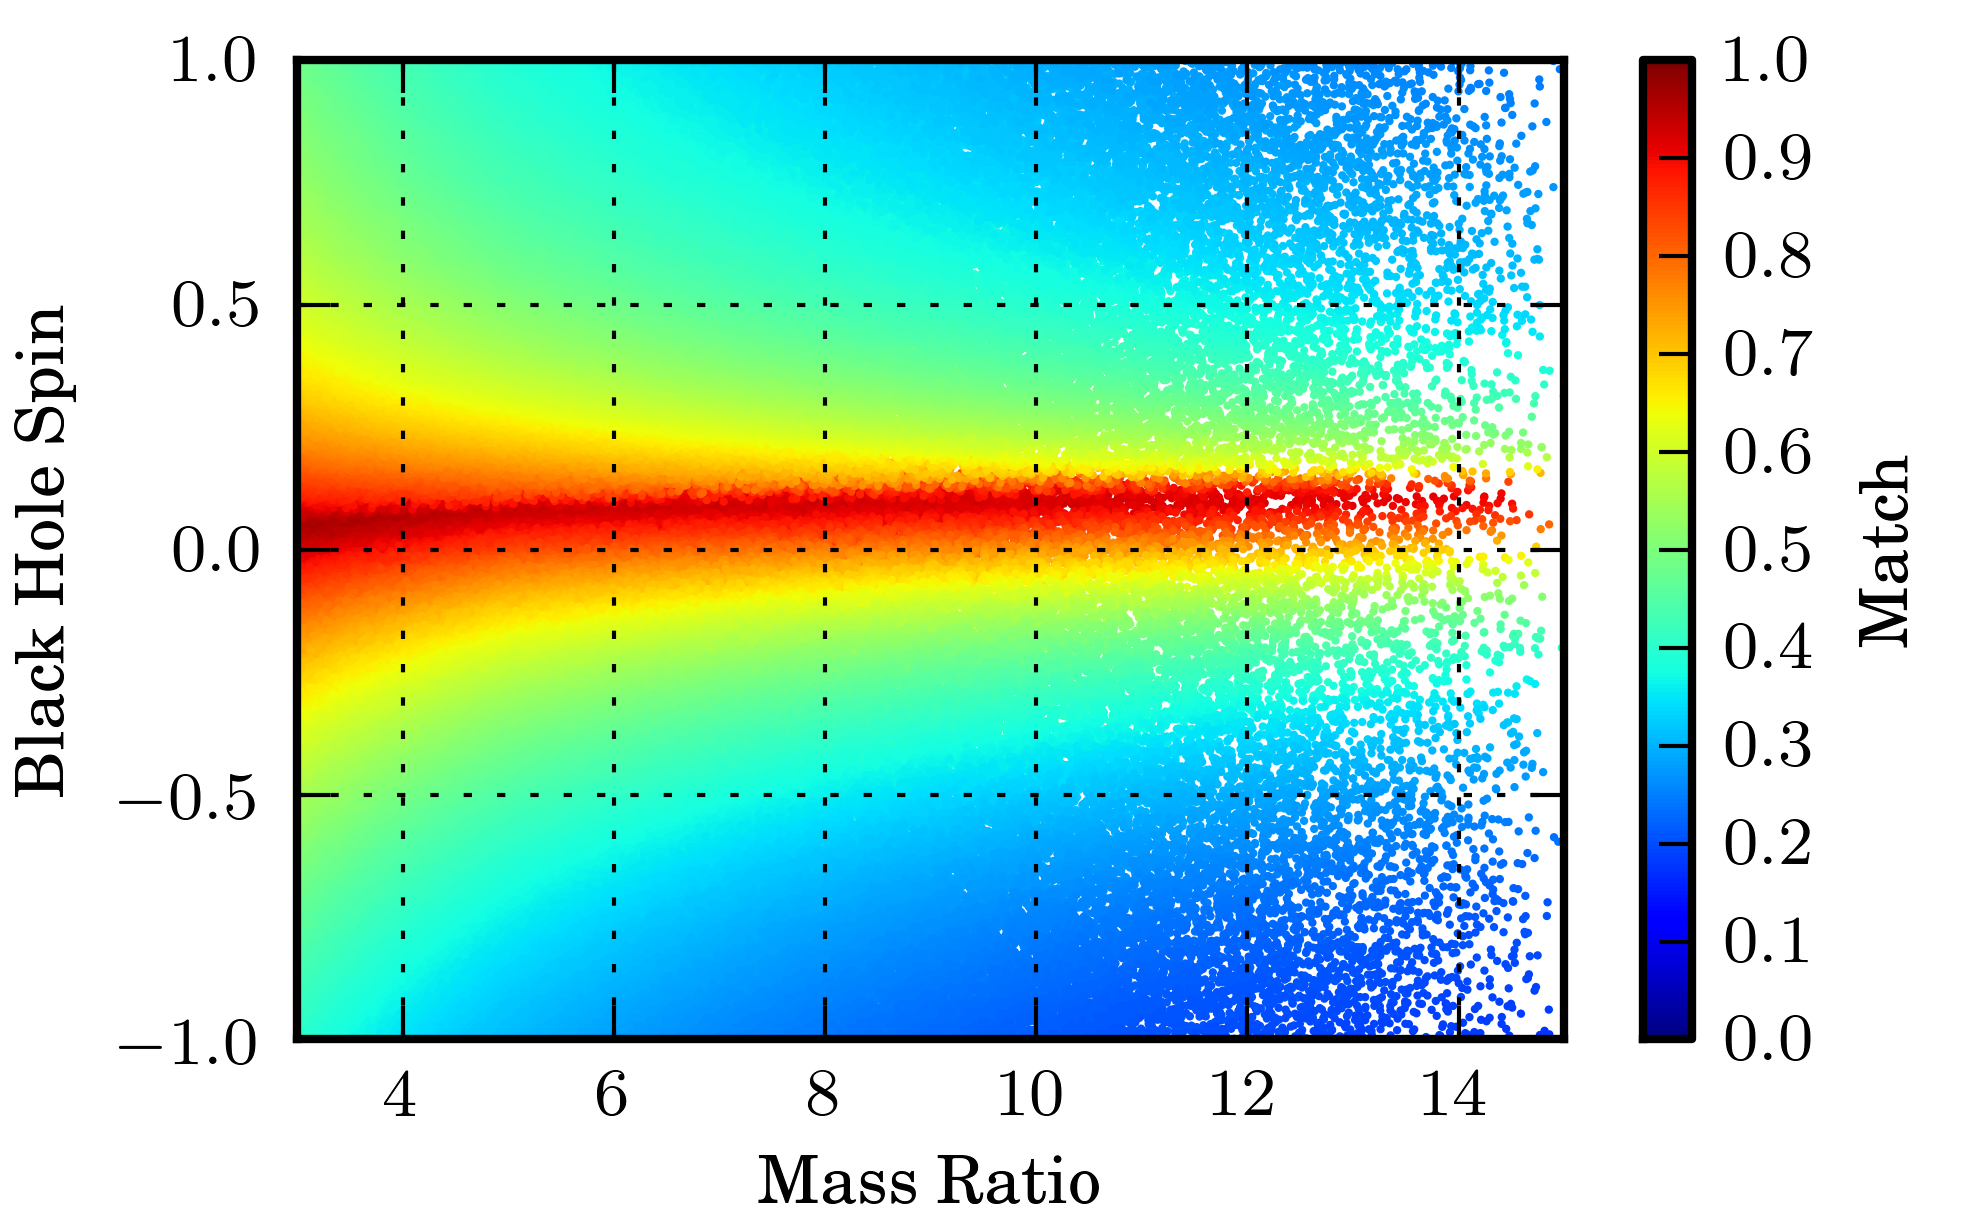
\includegraphics[width=1.0	\textwidth]{papers/nsbh_faithfulness/figure15.png}
\end{center}
\caption{\label{fig:5f2t430}The match between TaylorF2 and
TaylorT4 as a function of the spin of the black hole
and the mass ratio of the system. The approximants include spin corrections up to 2.5\ac{PN}. 
Matches are calculated using a 30Hz lower frequency cutoff to
approximate the sensitivity of an early \ac{aLIGO} detector. In comparison to Fig.~\ref{fig:f2f4f}, which uses a 15Hz lower
frequency cutoff, there is only a negligible improvement in match. Matches remain low at moderate black hole spins
$\chi \sim 0.3$.}
\end{figure}

\begin{figure}
\begin{center}
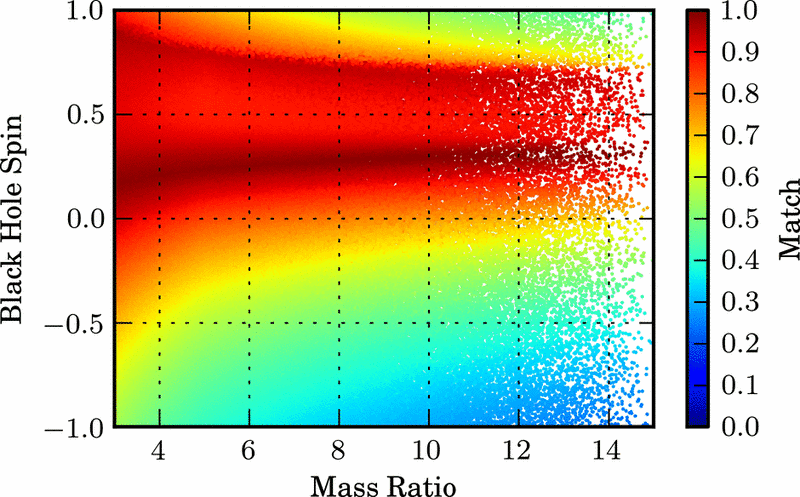
\includegraphics[width=1.0\textwidth]{papers/nsbh_faithfulness/figure16.png}
\end{center}
\caption{\label{fig:7f2t430}The match TaylorF2 and
TaylorT4 approximants, with the 3.5\ac{PN} spin-orbit and 3.0\ac{PN} spin-orbit tail corrections
included, as a function of the spin of the black hole
and the mass ratio of the system.  The approximants include only the nown
spin terms up to 2.5\ac{PN}. Matches are calculated using a 30Hz lower frequency cutoff to
approximate the sensitivity of the early \ac{aLIGO} detector. In comparison to Fig.~\ref{fig:f2t4fso}, which uses a 15Hz lower
frequency cutoff, there is only a negligible improvement in match. }
\end{figure}

In the previous sections we have modeled the sensitivity of aLIGO
with the 
zero-detuned, high-power sensitivity curve~\cite{aLIGOSensCurves}. 
Early commissioning scenarios for \ac{aLIGO}
indicate that observations will begin with less sensitivity in the 10--40~Hz
region~\cite{Aasi:2013wya}. We investigate if the substantial disagreement found between TaylorF2 and TaylorT4 is still present for 
early detector sensitives by a instead using a lower frequency cutoff of 30 Hz. 

In Fig.~\ref{fig:5f2t430} and~\ref{fig:7f2t430}, we show the faithfulness between the TaylorF2 and TaylorT4 
approximants that include only the complete 2.5~\ac{PN} and partial 3.5\ac{PN} spin-related corrections, respectively. 
We see that there is no significant improvement in the faithfulness of the approximants,
and so additional spin corrections are desirable even for early detector scenarios. 

\vspace{0.5cm}
%%%%%%%%
\section{Conclusions}

We have found that there is significant disagreement between \ac{NSBH}
waveforms modelled with the TaylorT2, TaylorT4, and SEOBNRv1 approximants. 
This will pose problems for the construction of optimal NSBH detection searches, 
potentially reducing the event rate, 
and may cause significant biases in the parameter measurement of detected signals.

The discrepancies are not accounted for by the differences between
frequency and time domain waveforms and start at fairly low ($v \sim 0.2$) orbital velocities.
Since the discrepancies in the approximants result from how the \ac{PN} expansions of the energy and flux
are combined and truncated, we conclude
that the calculation of higher order \ac{PN} terms is required to increase the
faithfulness of these approximants, and more importantly, to improve the
ability to detect \ac{NSBH} coalescences. The
discrepancies between approximants are significantly smaller when the spin of
the black hole is close to zero, which further motivates the calculation of the
\ac{PN} terms associated with the spin of the objects beyond those known
completely up to 2.5\ac{PN} order and partially up to 3.5\ac{PN}.
Therefore, additional work is needed to verify
the validity of waveform models used for \ac{NSBH} searches.
We also note that we have
only compared different waveform families under the assumption that the spins
of the component objects are (anti-)aligned with the orbital angular momentum
of the system.  It is expected that generic \ac{NSBH} systems will not be limited to
aligned spins, but may instead be more isotropically oriented.
This could lead to an additional source of discrepancy between our models and
the true signal, which would result in an additional loss in the detection rate
of sources.
